\documentclass[a4paper]{article}

\usepackage[english]{babel}
\usepackage[utf8]{inputenc}
\usepackage{amsmath, amssymb}
\usepackage{graphicx}
\usepackage[round]{natbib}
\usepackage{comment} 
\usepackage[margin=3cm]{geometry} %reduces margin
\linespread{1.6}
\usepackage{booktabs} %for tables
\usepackage{lscape}
\usepackage{chngpage} % fit table to page
\usepackage{bm}
\usepackage{tabularx}
\usepackage{tabulary}
\usepackage{caption}
\usepackage{subcaption}
\usepackage{hyperref}
\usepackage[symbol*]{footmisc}
\hypersetup{
    colorlinks,
    citecolor=black,
    filecolor=black,
    linkcolor=black,
    urlcolor=black
    linktoc=all
}



\begin{document}
\begin{titlepage}
\title{Mobile Money and Risk Sharing Against Aggregate Shocks}
\author{Emma Riley \footnote{I would like to thank  Karlijn Morsink, Simon Quinn and Climent Quintana-Domeque for their generous help, inspiring discussions, insight into economic research and assistance in helping me work through different ideas and econometric techniques. I would like to thank Tavneet Suri for her discussions around mobile money services and advice on data sources. I would like to acknowledge the LSMS division of the World Bank and the Tanzania National Bureau of Statistics for the main data used in this paper and for helping me with additional data needs.} \\ Department of Economics, Manor Road Building, Oxford OX1 3UQ, UK \\ (email: emma.riley@economics.ox.ac.uk)}
\thispagestyle{empty}
\maketitle 
\begin{center}
\section*{Abstract}
\end{center}
Households in developing countries have gained increased access to remittances through the recent introduction of mobile money services. While the benefits of improved risk sharing to the remittance receiver have been examined in past research, benefits to the wider community have not been looked into. I examine the impact of mobile money services on consumption smoothing after an aggregate shock for both users of mobile money and for household that don't use mobile money but who reside in villages with users. This allows me to determine the extent that remittances received via mobile money are shared within villages in which I cannot reject perfect risk sharing. Using a difference-in-difference fixed effects specification, I find that while having other mobile money users in the village increases the per capita consumption of the entire village, after an aggregate shock it is only users of mobile money who are able to prevent a drop in their consumption.  \\

\noindent Keywords: risk sharing, mobile money, Tanzania \\
JEL Classification - O16, O17, O33
\thispagestyle{empty}



\end{titlepage}

\setcounter{page}{1}
\newpage
\section{Introduction}
In developing countries, households use informal risk sharing networks to smooth their consumptions in response to unanticipated idiosyncratic shocks. Households within a village can insure their idiosyncratic shocks through  cross-sectional risk sharing. Cross-sectional risk sharing allows a household in a village who is affected by a shock to receive transfers from those who aren't affected. This is on the assumption that when the shocks are reversed a transfer will be made the other way and crucially relies on not everyone in the same village being subject to the same shock at once. Once village income is controlled for, this means that household income is partially or wholly insured against idiosyncratic income shocks, assuming no information or enforcement constraints (Townsend 1994, Udry 1994, De Weerdt \& Dercon 2006, Kazianga \& Udry 2006). Household consumption will depend on total village consumption, not household income. 

However, in reality village consumption is still affected by aggregate shocks which affect everyone in the village at once, against which the village is unable to self-insure itself. Larger risk sharing networks of friends and families in other villages could be used to insure this risk, such as in the case of remittances, but in practice it is costly and difficult to send money long distances due to high transaction costs. Mobile money services are a new tool allowing small amounts of money to cheaply, quickly and safely be sent around the country via a mobile phone, dramatically increasing access to a wider remittance network that households can draw from. By allowing risk sharing outside the village with people in other communities which will not have experienced the same aggregate shock, mobile money allows households to insure themselves against aggregate shocks.   

Under the assumption of perfect risk sharing, any remittances received by a household via mobile money would be shared with other members of the village, helping everyone in the village smooth their consumption after an aggregate shock. Any departure from perfect risk sharing would allow the household using mobile money to smooth their consumption more than the rest of the village. By comparing users and non-users of mobile money in the same village I am able to determine the extent to which mobile money remittances are shared in the village risk sharing network and hence assess if there is any departure from perfect risk sharing.    

The principal question of interest here is how the introduction of mobile money services allow remittances to flow into a village after it suffers an aggregate shock and to what extent these are shared throughout the village, allowing all households within the village to smooth their consumption. By comparing households in village with and without mobile money, and within villages with mobile money, households that do and do not use mobile money services, I can quantify the benefits of mobile money to both the recipient and to the rest of the village. While previous work has looked at the impact of mobile money on the user, no one has yet looked at the potential benefits to other members of a village when a household uses mobile money. Likewise, previous work has not separated aggregate and idiosyncratic shocks, while I argue a key contribution of mobile money services is enabling risk sharing when an entire village experiences a shock at once. This paper will build upon other work showing the benefit of mobile money use to the user after an idiosyncratic shock (Jack \& Suri 2014) and focus on the extent of sharing of the benefits of mobile money use within the village after an aggregate shock. 
 
Firstly, I show that households completely insure idiosyncratic shocks within the village, thus providing evidence for high levels of  risk sharing within the community. This builds upon other literature which has found significant consumption smoothing in response to idiosyncratic shock. Idiosyncratic shocks affect only one household at a time and are assumed to cancel out in terms of their impact on income in a sufficiently large community. I then look at aggregate shocks in the form of floods and drought, which are covariate, large and unexpected and hence cannot be insured within the village. I find that household consumption is significantly negatively affected, as predicted by the Mace (1991) model, with household consumption falling approximately 5\%.  

Secondly, I show that mobile money provides insurance against these aggregate shocks, resulting in household consumption of users no longer being negatively impacted by an aggregate shock. Mobile money therefore means that the classic Mace model result that household consumption moves with aggregate consumption no longer holds when households use mobile money. The mechanism proposed here is that mobile money allows the user access to remittances. When a user experiences an aggregate shock which cannot be insured at the village level, they can ask for help from family and friends in other locations which have not experienced a negative shock and with whom they can reciprocally insure. Remittances can then be sent easily and cheaply via mobile money. This means users of mobile money are able to smooth their consumption after an aggregate shock in a way non users aren't able to. This confirms the similar finding on mobile money in Kenya by Jack and Suri (2014).   

Thirdly, I  examine the wider impact of mobile money transfers within a village, something that has not been looked at before in previous work. In a world of perfect risk sharing within the village, if any household  uses mobile money and receives remittances after an aggregate shock this will be shared with other members of the village.  Receiving remittances therefore increases  insurance for the village as a whole. Hence consumption of non-mobile-money users in villages with other mobile money users will also not decline as much after an aggregate shock as that of households in villages without mobile money.

I find a significant and positive effect of having more mobile money users in the village on the consumption of everyone else in the village, suggesting that when an aggregate shock has not occurred remittances are being shared throughout the village, benefiting everyone. This is the first time a piece of work has placed the use of mobile money into the wider context of risk sharing in a village. However, while the user of mobile money is able to perfectly smooth the impact of an aggregate shock, non-users in villages with mobile money still experience a fall in consumption. Users of mobile money are not sharing their remittances with other members of the community after an aggregate shock. The fact that remittances are being shared when an aggregate shock hasn't occurred, but that the user of mobile money is choosing to insure their own consumption after an aggregate shock, is an interesting result in a village where I cannot reject that perfect risk sharing is occurring. Possible explanations for this are that recipients of mobile money are able to keep their remittances hidden, or they are choosing not to participate in the village risk-sharing network and instead relying on the stream of remittances for insurance. I discuss these more extensively in the Conclusion section. 

The remainder of this paper is organised as follows: I first survey the literature on both informal risk sharing and the emerging literature on mobile money services and their context in Tanzania. I then go through a simple model of how remittances can be included into the Mace (1991) model, outline the empirical specifications and make 6 predictions to be tested in the data. Section 3 summarises the data used in this paper and section 4 covers the  main results, robustness checks and mechanisms. Finally I conclude.  




\subsection{Literature review}


\subsubsection{Risk sharing}
The literature on the use of mobile money services to smooth consumption ties into a larger literature on how households share risk cross-sectionally. Therefore I begin by looking at why households share risk within a village and under what conditions risk sharing has been shown to work, before looking at the literature on when risk sharing fails. Last I look at wider risk sharing networks outside the village and the role of remittances. 

Households in developing countries are subject to a large amount of variability in income \citep{derconkrishnan1996}, particularly those reliant on agriculture. In response to this, households have developed strategies for reducing the impact of shocks. These include cross sectional strategies such as informal risk sharing as well as temporal strategies such as income diversification and asset accumulation/de-accumulation \citep{dercon2002}. In this paper the focus is on cross-sectional risk sharing.  

Under perfect risk sharing, the Pareto efficient outcome results in household income being a monotone increasing function of aggregate village income, so that household transient changes in income are perfectly pooled at the village level \citep{bardhanudry1999}. With complete markets this Pareto outcome can be achieved by any competitive equilibrium. However, complete markets are unlikely in the presence of information asymmetries and enforcement constraints which prevent credit and insurance markets working. 

A large body of research has shown that consumption is at least partially insured at the village level, supported by informal risk networks through mechanisms such as reciprocity within family and community networks. \cite{Townsend1994} finds that household consumption co-moves with village average consumption and isn't affected by factors like contemporaneous own income, sickness, unemployment or idiosyncratic shocks controlling for village consumption. However, he doesn't find that the full Pareto efficient outcome of risk sharing is achieved. \cite{chiappori2014} find that gifts and insurance transfers through family is the channel for risk sharing in the village and they are unable to reject full risk sharing in Tanzania villages where kin were also present, but strongly reject it when kin were not present. \cite{deweerdtdercon2006} look at detailed data on a village in Tanzania and the different risk sharing networks present. In response to illness shocks, they are unable to reject full risk sharing for food consumption and find at least partial insurance for non-food consumption via networks within the village.  

However there is also a body of work finding little or no risk sharing either at the village or household level. \cite{kaziangaudry2006} find far from complete consumption smoothing in Burkina Faso during a severe drought. They find almost no risk sharing in the village even to the idiosyncratic component of the drought and instead households rely almost exclusively on self insurance in the form of grain sales to smooth consumption in a limited way. Likewise \cite{udry1994} rejects perfect risk sharing in northern Nigeria in informal loan markets. \cite{ravallion1997risk} question the specification used in \cite{Townsend1994} and highlight the importance of measurement error, concluding there is strong evidence against perfect risk sharing. Even within the household, risk sharing is not complete, with wives experiencing reduced nutrition after a shock \citep{derconkrishnan2000}.

While idiosyncratic shocks can be insured at the village level, aggregate shocks will still impact village consumption and hence household consumption \citep{mace1991full}. A recent literature has examined the impact of offering rainfall insurance as a means to insure village consumption against aggregate shocks. \cite{mobarakrosenzweig2012} show that caste networks provide informal insurance against aggregate shocks and this lowers the demand for formal rainfall insurance. \cite{karlanudry2012} find that uninsured risk is the main impediment to farmers taking on more risky but higher returns investments and that this risk can be overcome by offering a rainfall insurance device.  

Networks of family and friends outside a household's own village are important for smoothing aggregate shocks which cannot be insured within the village. A number of papers have examined these links to others outside the village and how households share risk across a larger network. \cite{rosenzweig1988} finds that how well households are able to smooth risk ex post doesn't depend on the performance of the village economy but on the extent household have network links with other villages. \cite{fafchampslund2003} find that households do not receive insurance at the village level but instead mainly insure themselves through networks of family and friends. Shocks are principally insured through informal, state-contingent loans and pure transfers rather than through asset sales. These studies highlight how important networks outside the household's own village are for risk-sharing. 

Remittances are a channel through which households with family members outside the village can insure their consumption. \cite{yangchoi2007} look at remittance patterns in the Philippines, finding that remittances move in opposite directions to income with 60\% of the decline in income after a rainfall shock compensated for by increased remittances. Households without migrant members experience a fall in consumption.  \cite{yang2008}, looking at exchange rate shocks in the Philippines, finds that an increase in the value of remittances due to an appreciation of the migrant currency results in more remittances and that these are invested in businesses and child education.  

However, sending money across long distances by traditional channels such as through friends or via Western Union can be very costly, slow and unsafe, limiting the effectiveness of this channel. Mobile phone money transfer technology has the potential to overcome these barriers to sending remittances and lower costs \citep{JackSuri2014}, allowing users access to their wider risk-sharing networks and assisting households in smoothing aggregate shocks. 

\subsubsection{Mobile Money Services}
Even though mobile money services have been recently introduced, there is a growing literature on their impact, particularly on remittances and household consumption smoothing. Mobile money has expanded quickly since the launch of the first such service, M-Pesa, in Kenya in 2007. According to a report from the World Bank in 2012\nocite{WBfinancialinclusion}, in Kenya, 68\% of people were mobile money users, whereas the share in the rest of Sub-Saharan Africa was 16\% and in Tanzania 23\%. The quick growth of mobile money has allowed millions of people in developing countries who were otherwise excluded from the formal financial system to transfer money instantly from one phone to another at very low cost. The literature on mobile money is still small, with the first pieces of work focused on describing the patterns of use of mobile money services and how they affect remittance patterns, with recent work exploring the impact of mobile money using panel data. Previous work has focused on Kenya as the initial launch place of mobile money services. 

The early literature on mobile money focused on describing its use and correlations with other forms of banking or ways of sending remittances. \cite{MbitiWeil2011} describe the impact of M-Pesa in Kenya, finding that M-Pesa changes the pattern of remittance by increasing the frequency and volume of urban-rural transfers while lowering the price of competing remittance services such as Western Union. They  find 25\% of people report using M-Pesa for savings, and that it lowers the probability of people using informal saving mechanisms, such as ROSCAS, while raising the probability of them being banked. \cite{JackSuri2011} also look descriptively at the use of M-Pesa for sending remittances in Kenya and find that remittances sent via M-Pesa are less likely to go to parents and more likely to go to friends and other relatives  than other forms of remittance. This could signal that M-Pesa users have/take advantage of a broader network than non-users. They also find over 75\% of people use M-Pesa for savings. For those who don't use M-Pesa, the most commonly given reason is not owning a mobile phone followed by not needing the service. Less than 1\% report not having access to an agent. 

More recent papers have used panel data to determine the impact of mobile money services and particularly look at how sending remittances via mobile phones can help households respond to shocks. \cite{JackSuri2014} use panel data to analyse how mobile money facilitates consumption smoothing in response to negative idiosyncratic income shocks. They find that while the consumption of non-user households falls by 7\%-10\% after a shock, there is no corresponding fall for user households. They find that this effect is due to the improved ability to smooth risk via remittances; in the face of a negative shock, user households are 13\% more likely to receive any remittances, receive more remittances and receive a larger total value amounting to 6-10\% of annual consumption. Their proposed channel is that mobile money services reduce transaction costs and hence expand the number of network members a household can receive remittances from.   

\cite{blumenstock2014evidence} look at detailed transactional data on mobile airtime \footnote{Sending mobile airtime is an earlier, simpler service than mobile money but also allows the transfer of funds between two people via a mobile phone in the form of call balances. However it is much harder to turn the transferred funds into cash and can only informally be done} sent via mobile phones after an earthquake in Rwanda and find that mobile phones reduce transaction costs and enable Rwandans to share risk quickly across long distances. However they also find that wealthier people are more likely to receive transfers after the earthquake suggesting regressive consequences to the rapid uptake of mobile money service. They also show that the pattern of remittances is most consistent with a model of reciprocal risk sharing, where transfers are determined by past reciprocity and geographical proximity rather than one of pure altruism where transfers would be expected to be increase in the wealth of the sender and decreasing in the wealth of the recipient.

\cite{munyegera2014} look at the impact of mobile money services on household welfare using panel data from Uganda, finding wider benefits to household consumption than just the smoothing of shocks. They find that adopting mobile money increases per capita consumption by 69\% and that the mechanism for this is again through remittance. Households with mobile money are 20 percentage points more likely to receive remittances, receive remittances more frequently and the total value of the remittances received are higher 33\% than for non-user households. 

\cite{Batista2013} are the first to use an experimental design to assess the impact of randomised mobile money dissemination in rural Mozambique. They take advantage of the fact that the recent launch of mobile money allows the determination of a  control group. They randomised across 100 villages, with the randomisation determining which villages received an intense marketing campaign and recruitment of mobile money agents, and which individuals received an initial balance for signing up to the service. They found that 64\% of the individuals treated with mobile money made at least one transaction, while 81\% didn't withdraw the initial balance given to them when they signed up, consistent with an increase in general financial literacy and trust in the local agents. They also conducted a game to calculate the marginal willingness to send remittances, and find this increased 6-7\% in the treatment group compared to control. However, they didn't focus on any wider benefits of using mobile money or of the sending of remittances, such as increased risk sharing, as a savings instrument or to facilitate transactions. More randomised trials to help  determine the causal impact of mobile money services would be beneficial.  

The literature on mobile money is still new and growing, with initial papers describing the patterns of mobile money use and correlations. Other recent work has used panel data to look at the impact of mobile money on users and the channel this operates through, but there has yet to be any work on the wider impact of the service on non-users, or a more detailed analysis of the network links between senders and receivers. Randomised trials are difficult to carry out with a service like mobile money which is launched countrywide and there has only been one to date focusing on use of the service rather than benefits to the user. 


\input{Background_mobile_money_Tanzania}
\newpage
\section{Theoretical framework}
I start by setting out the canonical model of Mace (1991)  \nocite{mace1991full} to show how aggregate shocks impact household consumption. This is a simple framework which I use to show how household consumption varies with aggregate shocks. I then add an extension to this model by incorporating mobile money services as a flow of remittances to households. This allows me to determine three cases of the impact of aggregate shocks on consumption with and without mobile money services and with different degrees of village sharing of remittances.   

\subsection{Aggregate shocks}

As in the Mace model, I consider a village of risk-averse utility maximising households indexed by $j=1 \ldots J$. There are T periods and village states of nature $s_{\tau t}, \tau=1 \ldots S$. There is a probability $\pi(s_{\tau t})$ that state $\tau$ occurs in period $t$ such that $\sum_{\tau=1}^{S} \pi(s_{\tau t})=1$.  Each household has utility $U(C^j(s_{\tau t}),h^j(s_{\tau t}))$ where $C^j_t(s_{\tau t})$ is consumption and $h^j(s_{\tau t})$ is a preference shock representing changes in taste for consumption and both can be functions of the state of the world over time. I assume each household receives an exogenous amount of the consumption good $y_t^j(s_{\tau t})$ which is visible to everyone in the community. Households have no access to savings or credit. 

Mace showed that for the Pareto efficient outcome to be achieved:
\begin{equation} \label{eq: FOC1}
\frac{U'(C^i_t(s_{\tau t}))}{U'(C^j_t(s_{\tau t}))}=\frac{\lambda^j}{\lambda^i} \qquad \forall i, j, \tau, t
\end{equation}
where $\lambda^i$ is the welfare weight for household $i$. This condition says that the weighted marginal utilities are equated across households so that any household's consumption is a monotonically increasing function of average village consumption. 

I consider Mace's second class of utility functions, the power utility functions, that exhibit constant relative risk aversion \citep{Chiappori2011}: 
\begin{equation}
U(c,h)= \exp{\sigma h^j_t}\frac{1}{\sigma}(C^j_t)^{\sigma}
\end{equation}
Applying this utility functional form to the first order condition \eqref{eq: FOC1} aggregating over $J$ households and taking logarithms gives the consumption for a household as:
\begin{equation} \label{eq: consumption}
\ln C_t^j(s_{\tau t}) = \ln C^a_t(s_{\tau t}) + \frac{1}{1-\sigma}(\ln \lambda^i- \lambda^a) + \frac{\sigma}{1-\sigma}(h^i- h^a_t(s_{\tau t}))
\end{equation}
where
\[
C_t^a=\frac{1}{J} \sum_{j=1}^J \ln C_t^j \qquad \lambda^a=\frac{1}{J} \sum_{j=1}^J \ln \lambda^j \qquad  h^a_t=\frac{1}{J} \sum_{j=1}^J \ln h_t^j
\]
Mace showed that household consumption depends on aggregate consumption in the village plus a time invariant household fixed effect $\lambda$, which depends on the relative weight in the Pareto optimum allocation, and preference shifters. Household shocks are perfectly insured at the village level and do not affect household consumption. As mentioned in the initial assumptions, households have no savings in this model. This is to allow deviations from perfect risk sharing to be examined. While in reality households use other methods to smooth their consumption such as savings and credit, these can be controlled for in the empirical specification. 

I am interested in aggregate shocks, therefore I decompose the individual endowment of each household into its deterministic income, aggregate shock and idiosyncratic components assuming these are independent of each other:
Household $j$ receives an exogenous endowment of the consumption good $y^j_t(s_{\tau t})$ which is visible to everyone in the village. This can be decomposed into the deterministic and stochastic components: 
\begin{equation} \label{eq: endow}
y^j_t(s_{\tau t}) = \bar{y}^j_t + \eta_t^j(s_{\tau t}) + \epsilon_t^j(s_{\tau t})
\end{equation}
where $\bar{y}^j_t$ is the deterministic portion of output, $\eta_t^j(s_{\tau t})$ is an aggregate shock to household $j$'s endowment (which may still differ across households) and $\epsilon_t^j(s_{\tau t})$ is the idiosyncratic shock experiences by household $j$ only. When equation \eqref{eq: endow} is aggregated across $J$ households the aggregate endowment is given by:
\begin{equation} \label{eq:agg endow1}
y^a_t(s_{\tau t}) = \bar{y}^a_t + \eta_t^a(s_{\tau t})
\end{equation}
where 
\[
y^a_t(s_{\tau t})= \frac{1}{J}\sum_{j=1}^Jy^j_t(s_{\tau t}) \qquad \bar{y}^a_t= \frac{1}{J}\sum_{j=1}^J \bar{y}^j_t \qquad  \eta^a_t=\frac{1}{J}\sum_{j=1}^J\eta_t^j(s_{\tau t}) \qquad \sum_{j=1}^J \epsilon_t^j(s_{\tau t})=0
\]
Idiosyncratic shocks balance out within the village as J approaches infinity. Aggregate uncertainty means $\eta_t^a(s_{\tau t}) \neq 0$ for at least one event for all $t$. The aggregate resource constraint says that $C^a_t=y^a_t$ therefore I can substitute \eqref{eq:agg endow1} into equation \eqref{eq: consumption}. 
\begin{equation} \label{eq: agg shock}
\ln C_t^j(s_{\tau t}) = \ln (\bar{y}^a_t + \eta_t^a(s_{\tau t})) + \frac{1}{1-\sigma}(\ln \lambda^i- \lambda^a) + \frac{\sigma}{1-\sigma}(h^i- h^a_t(s_{\tau t}))
\end{equation}
Household consumption depends on the deterministic component of village consumption $\bar{y}$, an aggregate shock $\eta$, a household fixed effect and preference shifts. Idiosyncratic shocks are perfectly insured by the village as $J \rightarrow \infty$. However, for a village in which all households experience the same aggregate shock at once, consumption will fall. 

\subsection{Mobile money}
The above section showed how household consumption depends on aggregate shocks. I will now combine this with mobile money services and look at how mobile money allows remittances from someone outside the village to respond to the aggregate shock. I will consider mobile money users, non-users in villages with mobile money and non-users in villages without mobile money. 

I consider an economy in which households can only share risk with each other when there is a social tie between them. Households have social ties both with households within their own village but also with households outside their village, for example if a member of their household leaves the village to work in another village or the city (a migrant). Having links with people outside the village in far away locations increases the diversification of income streams across the risk sharing network. The set of social networks is taken as given. With no constraints on commitment or enforcement and the network connected (so that everyone is linked up in the network), risk sharing will be efficient. However, if networks are closed such that different networks are not linked then exchange is limited to members of one's own network. 

I assume that transfers can only take place via mobile money payments so that only households that use mobile money can receive remittances after an aggregate shock. Aggregate shocks are assumed to not be perfectly correlated across locations so that reciprocal transfers are possible between different locations undergoing shocks at different times. If there is at least one household in a village that receives a transfer via mobile money, this will be shared with everyone else in the village due to the perfect risk sharing assumption discussed above. 
Members of a village who don't use mobile money themselves but with at least one mobile money user can receive transfers from the mobile money using household. In a perfect risk sharing world, a recipient of remittances is assumed to share these perfectly with other members of their risk sharing network. Remittances therefore provide insurance to the entire village and dampen the negative effect of the aggregate shock.

As an example, suppose there are three households, $A$, $B$ and $C$.  Households $B$ and $C$ both reside in the same village, but $A$ is in another village far away. Household $B$ is connected to both households $A$ and $C$ in a risk-sharing network and so able to facilitate exchange with both of them. If $B$ and $C$ experience an aggregate shock in their village, $A$ can send transfers to them through $B$ via mobile money. $B$ will then share any remittances with $C$ and so dampen the impact of the aggregate shock for both. 

Expanding this model to many households within each village, mobile money use can be seen to connect the village risk sharing network to households outside the village. The more mobile money users there are in a village, and the more connections these households have to households in other villages, the more smoothing there will be of consumption after an aggregate shock. I assume that the sender of remittances has past information about the size of losses after aggregate shocks and so sends an amount equal to the average of these losses. Assuming the majority of remittance senders were once living in the household as children, they should have an idea of how large losses would be in the event of a shock and send an amount expected to cover this.  Households who don't use mobile money themselves can only receive transfers from the households within their village that do use mobile money. For example, the amount of transfers that household $C$ receives will be increasing in the proportion of other households in the village who use mobile money, assuming they are linked to different migrants who send them remittance. 

I can also use this as a test of the degree that remittances are shared perfectly within a village. If the recipient of the mobile money does not share the remittance with other members of the village, then that household will better smooth its income after the aggregate shock than other households in the village, and this can be tested in the data. Possible reasons for not sharing the remittance are being able to hide the remittance from other members of the village or because the household with a migrant member chooses to insure itself through that network instead of through the village risk sharing network. 

If there are two other households, $D$ and $E$, who are located in different villages but not connected to each other via mobile money, when $E$'s village suffers from an aggregate shock, $D$'s village will be unable to insure it. 

This gives 3 cases for the impact of an exogenous rainfall shock which I will formalise as: 

\textbf{Case 1: No mobile money use}. Non-users in villages without mobile money will experience the full negative impact of the aggregate shock $\eta_t^a(s_{\tau t})$  on each household's consumption as in equation \eqref{eq: agg shock}.  Suppose there are two villages with a migrant in village 1, D, and a home network village 2 which experiences a rain shock. Without any links to D in village 1, the households of village 2 will experience a drop in consumption since they are unable to insure themselves against the aggregate shock. 

\textbf{Case 2: Perfect village sharing}. In villages with mobile money, I assume $M$ users of mobile money and $N$ non-users such that $N+M=J$. Users of mobile money receive a transfer $t^m$ which is insufficient to cover the impact of the aggregate shock for the entire village, $t^m<J\eta_t^a(s_{\tau t})$ but can cover the aggregate shock for one household $t^m=\eta_t^a(s_{\tau t})$. With $M$ mobile-money-using households each receiving a transfer $t^m$ and shared between $J$ households, each household receives $\frac{M}{J}t^m$. 

It can be seen that all households are partially insured against the aggregate shock by $\frac{M}{J} t^m<\eta_t^a(s_{\tau t})$ which increases proportionately to the number of mobile-money-using households in the community such that if all households use mobile money and receive remittances the aggregate shock would be completely insured against. All households will get consumption of:
\begin{equation} \label{eq: perfect sharing}
\ln C_t^j(s_{\tau t}) = \ln (\bar{y}^a_t + \eta_t^a(s_{\tau t}) + \frac{M}{J}t^m) + \frac{1}{1-\sigma}(\ln \lambda^i- \lambda^a) + \frac{\sigma}{1-\sigma}(h^i- h^a_t(s_{\tau t}))
\end{equation}

To illustrate, suppose the migrant worker in village 1, $A$, is linked via mobile money to household $B$ in village 2. When village 2 experiences a rainfall shock, household $A$ sends money to household B who then shares this with all the other households in the village, such as $C$. Hence there are benefits in mobile money use to the rest of the community. Every household experiences a small drop in consumption due to the aggregate shock since $A$ cannot insure the entirety of village 2. The amount of insurance will be increasing in the number of distinct links to migrants in outside villages. 

\textbf{Case 3: The mobile-money-using household does not share the remittance with other households in the village.}
The mobile money using household receives the transfer $t^m$ and does not share this with the rest of the community,  but uses it itself to smooth the aggregate shock. Whatever the reason for the household not sharing the remittances, if remittances are not shared there will be no consumption smoothing benefit from mobile money users to other members of the community.  Mobile-money-using households will get consumption of:
\begin{equation} \label{eq: MM users}
\ln C_t^j(s_{\tau t}) = \ln (\bar{y}^a_t + \eta_t^a(s_{\tau t}) + t^m) + \frac{1}{1-\sigma}(\ln \lambda^i- \lambda^a) + \frac{\sigma}{1-\sigma}(h^i- h^a_t(s_{\tau t}))
\end{equation}
where the transfer $t^m$ exactly counters the negative aggregate shock $\eta^a$.

For example, if village 2 experiences a rainfall shock, household $A$ sends money to household $B$, compensating the household for any drop in consumption due to the aggregate shock. $B$ does not share this with other households in the village. Other households in village 2, will therefore still suffer a drop in consumption due to the aggregate shock.





\clearpage
\subsection{Identification strategy} 
In this section I use the previous theoretical framework to determine two estimating equations, the first of the extent of perfect risk sharing within the village and the second of the impact of mobile money use after an aggregate shock. 

\subsubsection{Specification 1: Village risk sharing of idiosyncratic shock}
I first want to determine if idiosyncratic risk is perfectly shared within the village. To do this I look at the impact of a variety of different household shocks on household per capita consumption, controlling for the level of village consumption. I run the following specification: 
\begin{align} \label{eq: idioshock}
C_{jvt} = &   \gamma_i IdioShock_{jvt}  + \bm{\theta X_{jvt}}   +  \delta_{vt} + \alpha_j + \varepsilon_{jvt} 
\end{align}
where $Idioshock_{jvt}$ is an idiosyncratic shock experiences by household $j$ in village $v$ at time $t$,  $\bm{X_{jvt}}$ is a vector of controls consisting of household demographics, financial service use and occupation dummies to control for other variables which allow households to smooth consumption, $\delta_{vt}$ are village-time dummies to control for village level variations, including variation of aggregate village consumption as in \cite{ravallion1997risk}, $\alpha_j$ is a household fixed effect picking up fixed characteristics of the household (including the Pareto weight) and $\varepsilon_{jvt}$ is a time varying error. If household risk is perfectly pooled within the village then idiosyncratic shocks should have no impact on household consumption once village consumption is controlled. This means that the coefficient on $IdioShock_{jvt}$ should be insignificantly different from zero: 
\begin{description}
\item{\bf{Prediction 1}} $\gamma_i=0$
\end{description}

I estimate this specification using a fixed effect regression with three waves of household panel data.

\subsubsection{Specification 2: Impact of mobile money use}
If mobile money allows for transfers to be made in response to an aggregate shock, then consumption will no longer respond to aggregate shocks. If these transfers are shared perfectly within the village then village consumption smoothing will depend on the proportion of mobile money users in the community and there will be a positive spillover to non-users from other members of the community using mobile money. If transfers are kept by the user of mobile money then only the user will be able to smooth consumption after an aggregate shock. In order to examine each of these potential impacts of mobile money, I first write equation \ref{eq: perfect sharing} as a specification I can estimate.  

Writing equation \ref{eq: perfect sharing} as an empirical specification, the aggregate shock $\eta^a_t$ can be captured by a measure of unexpected shocks affecting the whole village $AggShock_{jvt}$, the impact of being the recipient of mobile money transfer by a dummy for mobile money use $MM_{jvt}$, the impact of being in a village with $M$ mobile money users by a variable for the proportion of households in the village using mobile money $VMM_{vt}$, the pareto weight by a household fixed effect $\alpha_j$, the deterministic component of income $\bar{y}$ by household characteristics $\bm{X_{jvt}}$, and the preference shock for both individual households and in aggregate by an error term $\varepsilon_{jvt}$. This error term will also contain any measurement error. 
 

With these assumptions, the empirical specification can be written as:
\begin{align} \label{eq: specification agg shock}
C_{jit} = &  \gamma_a AggShock_{jvt} + \mu MM_{jvt}   +\lambda VMM_{vt}  \notag \\
&  + \beta_m MM_{jvt}\cdot AggShock_{jvt} +\beta_v VMM_{vt}\cdot AggShock_{jvt} \notag \\
& + \bm{\theta X_{jvt}} +  \bm{\psi X_{jvt}} \cdot AggShock_{jvt} +  \alpha_j + \delta_t + \varepsilon_{jvt} 
\end{align}
where $C_{jvt}$ is household $j$'s per capita log consumption in village $v$, $AggShock_{jvt}$ is a rainfall shock in village $v$, $MM_{jvt}$ is mobile money use by household $j$ in village $v$,$VMM_{vt}$ is the proportion of mobile money users in village $v$ at time t, $\bm{X_{jvt}}$ is a vector of controls consisting of household demographics, financial service use and occupation dummies to control for any other variables which might enable households to better smooth consumption, $\alpha_j$ is a household fixed effect, $\delta_t$ is a time trend and $\varepsilon_{jvt}$ is a time varying error. 

The parameters of interest are $\beta_m $,  which allows for use of mobile money to affect the household's ability to smooth shocks and $\beta_v$, which allows for the proportion of people using mobile money in the village to impact the household's ability to smooth shocks.

This gives the following predictions for the empirical estimation:
\begin{description}
\item{\bf{Prediction 2}} For households in villages without mobile money (when $MM_{jvt}=0$ and $VMM_{vt}$=0), $\gamma_a<0$ so that rainfall shocks have negative effects on consumption
\item{\bf{Prediction 3}} For households in villages with at least one mobile money user, if remittances are perfectly shared within the village then consumption smoothing after an aggregate shock will depend only on the proportion of mobile money users in the community. Greater consumption smoothing will take place the more users of mobile money there are in the community so that $\beta_v >0$. There will be no 
differential response to the aggregate shock for users of mobile money compared to other members of the same village who don't use mobile money once the number of mobile money users in the village has been controlled for, $\beta_m=0$
\item{\bf{Prediction 4}} If users of mobile money do not share remittances after an aggregate shock with other members of the village then $\beta_v=0$ and $\beta_m>0$. 
\end{description}

I estimate equation \eqref{eq: specification agg shock} using difference-in-differences on a household panel dataset. Difference-in-difference estimation attempts to mimic an experimental research design through the calculation of differences in the changes of a control and treatment group. In the panel data case, difference-in-difference subtracts the average change in the control group (households in villages without mobile money) from the average change in the treatment group (users of mobile money or non-users in villages with mobile money), therefore removing biases from permanent differences between the two groups and changes due to a time trend. The use of fixed effects allows for unobserved constant household characteristics to be removed and hence controls for selection effects. 

To estimate equation \eqref{eq: specification agg shock} using a difference-in-difference specification requires the common trends assumption. This assumes that there are no differences in the trends of users and non-users, had the users not actually used mobile money i.e. there are no time varying variables that differentially affect the mobile money using and non-using households. An example of such a violation would be local prices and supply side effects. The counterfactual levels for the two groups can be different but the time trends must be the same so that in the absence of the use of mobile money the change in per capita consumption would have been the same for the two groups. I test this by running a placebo test using pre-treatment data in the Robustness section.

For equation \eqref{eq: specification agg shock} to identify the impact of other members of a village using mobile money, $ AggShock_{jvt} \cdot MMV_{vt}$ must be uncorrelated with the error term. This means that unobserved factors which cause villages to have more members using mobile money cannot also help them smooth consumption following a shock. For the above specification to identify the impact of mobile money use on consumption smoothing, the interaction term $ MM_{jvt} \cdot AggShock_{jvt}$ must also be uncorrelated with the error term $\epsilon_{jvt}$. This means that unobserved factors which cause a household to use mobile money for smoothing shocks cannot also help them smooth consumption following a shock.  Household unobservables which don't change with time can be controlled for using a fixed effects specification, as shown by the inclusion of $\alpha_j$.

Fixed effects will account for time invariant unobservables but not for time varying unobservable characteristics e.g changing risk preference or changing technology preference which influence mobile money use and risk sharing capacity. Since there isn't  randomisation in mobile money take-up, the solution here is to instrument for mobile money use. In addition to instrumenting I also use propensity score matching to match mobile money users to a sample of non-users with as similar characteristics as possible. This will be covered in the Robustness section. 

\newpage
\section{Data and summary statistics}
\subsection{Household panel}
The data used comes from the Tanzania National Panel survey (NPS) 2008-9, 2010-11 and 2012-13, implemented by the Tanzania National Bureau of Statistics and downloaded from the World Bank LSMS microdata catalogue. The survey covers 3,265 households in 26 districts containing 409 Enumeration Areas (EAs), and is designed to be representative of Tanzania as a whole. Within each EA (village) 8 households were randomly selected. The survey made particular effort to track respondents, with all adult former households members tracked to new location, resulting in over 97\% of the round 1 households being re-interviewed in round 2 and a total panel attrition rate of 4.8\%. The data includes weightings of the probability that an observation was included in the survey to take into account the fact that some areas were over surveyed to reflect the higher variance of the variables of interest (for example in cities). 

 
% Table generated by Excel2LaTeX from sheet 'HH stats'
\begin{table}[htbp]

  \centering
  \caption{HH summary stats by wave} \label{HH sum}
    \begin{tabulary}{1\textwidth}{Lcccccc}
    \toprule
          & \multicolumn{2}{c}{Wave 1}        & \multicolumn{2}{c}{Wave 2} &      \multicolumn{2}{c}{Wave 3}   \\
    \midrule
          & Mean  & SD    & Mean  & SD    & Mean  & SD \\
    Per capita consumption &            743,386 &            725,334  &            862,266  &               782,264  &           1,011,279  &          1,090,465  \\
    Rural & 0.65  & 0.48  & 0.68  & 0.47  & 0.65  & 0.48 \\
    Rainfall shock & 0.09     & 0.28  & 0.09  & 0.29  & 0.20  & 0.40 \\
    wealthscore  & -0.11  &  3.00 & 0.14  &   2.85 & -0.05  &   2.56  \\
    Education of head (yrs) & 4.76  & 3.57  & 4.84  & 3.65  & 4.96  & 3.70 \\
    Age of head & 45.53 & 15.05 & 45.85 & 15.53 & 46.71 & 16.04 \\
    Head female & 0.25 & 0.43 & 0.26 & 0.43 & 0.28 & 0.446 \\
    Household size & 5.08  & 2.86  & 5.28  & 3.13  & 5.02  & 3.05 \\
    Mobile money use & 0.00  & 0.00  & 0.13  & 0.33  & 0.38  & 0.49 \\
    Own mobile & 0.45  & 0.50  & 0.62  & 0.48  & 0.71  & 0.45 \\
    \textit{Financial access } &       &       &       &       &       &  \\
    Number of loans & 0.07  & 0.30  & 0.10  & 0.35  & 0.12  & 0.39 \\
    Bank account & .     & .     & 0.20  & 0.40  & 0.20  & 0.40 \\
    ROSCA & 0.04  & 0.20  & 0.05  & 0.22  & 0.04  & 0.19 \\
    Wealth index & -0.80 & 2.99 & 0.14 & 2.84 & -0.89 & 2.56 \\
    \textit{Occupational dummies} &       &       &       &       &       &  \\
     Agriculture/ Livestock" & 0.60  & 0.49  & 0.56  & 0.50  & 0.55  & 0.50 \\
     Fishing & 0.02  & 0.14  & 0.01  & 0.12  & 0.01  & 0.12 \\
     Mining & 0.00  & 0.05  & 0.00  & 0.06  & 0.00  & 0.06 \\
     Tourism & 0.00  & 0.02  & 0.00  & 0.02  & 0.00  & 0.02 \\
     Employed: Government & 0.06  & 0.23  & 0.06  & 0.24  & 0.06  & 0.23 \\
     Parastatal & 0.01  & 0.08  & 0.01  & 0.08  & 0.01  & 0.07 \\
     Private sector & 0.09  & 0.28  & 0.11  & 0.31  & 0.12  & 0.33 \\
     NGO/religious & 0.01  & 0.09  & 0.01  & 0.08  & 0.01  & 0.09 \\
     Self-employed (non-agri) w employees & 0.02  & 0.16  & 0.03  & 0.18  & 0.03  & 0.16 \\
     Self-employed (non-agri) w/o employees & 0.15  & 0.35  & 0.14  & 0.35  & 0.15  & 0.36 \\
     Unpaid family work & 0.01  & 0.05  & 0.01  & 0.11  & 0.01  & 0.11 \\
     
     Job seeker & 0.00  & 0.05  & 0.00  & 0.07  & 0.00  & 0.04 \\
    
     Disabled  & 0.00  & 0.03  & 0.02  & 0.15  & 0.03  & 0.17 \\
     No job & 0.01  & 0.12  & 0.02  & 0.13  & 0.02  & 0.13 \\
    \hline
    \end{tabulary}%
  \label{tab:addlabel}%
\end{table}%
 

% Table generated by Excel2LaTeX from sheet 'HH stats'
\begin{table}[htbp]
  
  \centering
  \caption{HH Summary stats by mobile money adoption at wave 3} \label{HH adoption}
    \begin{tabulary}{1 \textwidth}{Lcccccc}
    \toprule
          & \multicolumn{2}{c}{Early adopters}       & \multicolumn{2}{c}{Late adopters} & \multicolumn{2}{c}{Non-Adopters} \\
    \midrule
          &  Mean  &  SD   &  Mean  &  SD   &  Mean  &  SD  \\
   
    Per capita consumption &          1,670,892  &          1,374,892  &          1,498,173  &          1,348,243  &               702,110  &          744,725  \\
    Rural &                     0.30  &                     0.46  &                     0.40  &                     0.49  &                      0.81  &                 0.39  \\
    Rainfall shock &                     0.15  &                     0.36  &                     0.16  &                     0.36  &                      0.22  &                 0.42  \\
    wealthscore & 2.23 & 3.07 & 1.24 & 3.04 & -0.94 & 1.74 \\ 
    Education of head (yrs) &                     7.57  &                     3.97  &                     6.58  &                     3.68  &                      3.93  &                 3.32  \\
    Age of head &                   44.49  &                   13.56  &                   43.62  &                   14.82  &                   48.62  &              16.50  \\
    Head female & 0.22 & 0.41 & 0.25 & 0.43 & 0.29 & 0.45 \\
    Household size &                     4.94  &                     2.74  &                     4.79  &                     3.01  &                      5.16  &                 3.06  \\
    Household wealth index &                     2.23  &                     3.07  &                     1.24  &                     3.04  & -                   0.94  &                 1.74  \\
    Mobile money use &                     0.88  &                     0.33  &                     1.00  &                          -    &                          -    &                     -    \\
    Own mobile &                     0.97  &                     0.18  &                     0.98  &                     0.15  &                      0.54  &                 0.50  \\
    \textit{Financial access } &       &       &       &       &       &  \\
    Number of loans &                     0.26  &                     0.52  &                     0.21  &                     0.50  &                      0.07  &                 0.28  \\
    Bank account &                     0.52  &                     0.50  &                     0.40  &                     0.49  &                      0.07  &                 0.26  \\
    ROSCA &                     0.09  &                     0.29  &                     0.07  &                     0.26  &                      0.02  &                 0.13  \\
    Wealth index & 2.32 & 3.65 & 1.33 & 3.31 & -0.81 & 2.00 \\
    \textit{Occupational dummies} &       &       &       &       &       &  \\
     Agri/ Livestock &                     0.28  &                     0.45  &                     0.34  &                     0.47  &                      0.68  &                 0.47  \\
     Fishing &                          -    &                          -    &                     0.01  &                     0.09  &                      0.02  &                 0.13  \\
     Mining &                     0.00  &                     0.05  &                     0.00  &                     0.07  &                      0.00  &                 0.05  \\
     Tourism &                          -    &                          -    &                          -    &                          -    &                      0.00  &                 0.02  \\
     Employed: Gov &                     0.13  &                     0.34  &                     0.10  &                     0.30  &                      0.03  &                 0.16  \\
     Parastatal &                     0.02  &                     0.15  &                     0.01  &                     0.09  &                      0.00  &                 0.05  \\
     Private sector &                     0.18  &                     0.38  &                     0.19  &                     0.39  &                      0.08  &                 0.27  \\
     NGO/religious &                     0.02  &                     0.13  &                     0.01  &                     0.12  &                      0.00  &                 0.05  \\
     Self-employed (non-agri) with employees &                     0.07  &                     0.26  &                     0.05  &                     0.22  &                      0.01  &                 0.10  \\
     Self-employed (non-agri) w/o employees &                     0.23  &                     0.42  &                     0.22  &                     0.41  &                      0.11  &                 0.32  \\
     Unpaid family work &                     0.01  &                     0.10  &                     0.01  &                     0.11  &                      0.01  &                 0.11  \\
    Job seeker &                          -    &                          -    &                     0.00  &                     0.04  &                      0.00  &                 0.04  \\
     
     Disabled  &                     0.02  &                     0.13  &                     0.02  &                     0.15  &                      0.03  &                 0.18  \\
     No job &                     0.03  &                     0.17  &                     0.02  &                     0.14  &                      0.02  &                 0.13  \\
    \bottomrule
    \end{tabulary}%
    \label{tab:addlabel}%

\end{table}%


The survey included questions on consumption, assets, finance, shocks, household characteristics and village characteristics, as well as detailed agricultural and fisheries information. I combined the data by household since mobile money use is only recorded at the household level. Looking at the characteristics of the household head in table \ref{HH sum}, the average household has 5 people, average years of education of the household head is just under 5 years, increasing slightly during the survey. 60\% of household heads worked in agriculture, 10\% in the private sector as paid worker and 15\% were self employed. In 2008-09 annual real per person consumption was 742,386 TZ Shillings (\$450), rising to 802,256 shilling (\$490) in 2010-11 and 1,011,279 (\$568) in 2012-13. 

I generated a wealth index of assets using principal component analysis (PCA). Different components of wealth, such as the number of chickens owned or bicycle ownership, cannot easily be added up. PCA determines the relative importance of variables when seeking to summarize a set of variables. It reduces the set of variables by comparing how similar they are to each other, and based on this creates a new variable called the principal component. The first principal component accounts for the largest variance across the variables. In a wealth index, the first principal component is assumed to represent relative wealth. Based on this, each factor is given a factor weight representing its relative importance in constructing the principal component. I generated a wealth index score based on these factor weights. 

Looking at mobile phone ownership and mobile money use,  in 2008-9, 45\% of households owned at least one mobile phone, increasing to 62\% in 2010-11 and 71\% in 2012-13. 13\% of households had used a mobile money service in 2010-11 and 38\% had by 2012-13. I am interested in both users and non users in villages with mobile money and non-users in villages without mobile money. Therefore I break down the number of villages and households by these categories in Figure \ref{fig:users chart}. This figure shows the large increase in both villages with mobile money agents and mobile money users within these villages. By the second round of the survey 17\% of the communities had a mobile money agent present within the village, and a further 21\% had mobile agents within 5km of the community. By 2012-13, 52\% of the communities had a mobile money agent and a further 13\% were within 5k of one.  
\begin{figure}
\centering
\includegraphics[width=\textwidth,trim= 0 3cm 0 3cm, clip=true, keepaspectratio]{users_chart_} 
\caption{Break down of villages and households by mobile money use} \label{fig:users chart}
\end{figure}

I also examine characteristics by adoption date of mobile money in Table \ref{HH adoption}. Early adopters used mobile money in the second round, 2010-11, and late adopters in the third round, 2012-13. A few people used mobile money in the second round but not in the third. Those who used mobile money are more educated, richer, more likely to live in an urban area and have a bank account and loans, almost always have a mobile phone and are slightly younger than those who don't use mobile money. They are less likely to work in agriculture and more likely to work in the private sector or be self employed. These differences are important to take into account when estimating the impact of mobile money use. 

Sending and receiving money are by far the most popular uses of mobile money, with 67\% of users saying they send money and 82\% of users saying they receive money. These two uses are also given as the most important use of mobile money services by 80\% of respondents. 40\% of people report using mobile money services to save up for emergencies or expenses and 12\% have used it to pay for a good or service. 40\% of people use the service at least monthly. The most common reasons for not using mobile money are no mobile phone, don't understand the service and lack of access to agent, with each of these given in just over a third of responses.  

In the third round of the survey there was detailed data on who sent the remittances to whom using what channel, where from and what their relationship was to the sender. 55\% of remittances were sent via friends and family and 50\% by mobile money. Only 3\% was sent using a bank account, 1\% using Weston Union and 0.4\% using the Post Office. In the past it's likely that the majority of remittances were sent via friends and family with very little sent using any more formal channels. 40\% of remittances were sent by a son or daughter with only 3.5\% sent via a spouse, 7\% by a parent and 17\% by a sibling. 30\% of remittances are sent from Dar Es Salaam. This is consistent with a pattern of a family member migrating to another location such as the city and then sending remittances back to their family. 


\subsection{Rainfall measure}
The panel data contains information on self reported shocks, including whether a household has experienced a drought or flood. This is a dummy equal to one if the household reported that they experienced a drought or flood in the year proceeding the survey wave. To the extent that households misreport or subjectively interpret a rainfall shock, for example saying they experienced a rainfall shock to justify a poor crop yield or exaggerating the importance of a rainfall shock in a year when they have no other shocks, this measure of rainfall shocks will be subject to bias and measurement error. I therefore also calculate a rainfall shock measure per village using data from the NOAA's climate prediction centre FEWS (Famine Early Warning System). This is available at 0.1 degree resolution by latitude and longitude across Africa and was included in the Tanzania NPS summarized at the EA level. 

I define a rainfall shock as more than a 1 standard deviation in absolute values from the 15 year mean by the nearest rainfall station to the village, as used in \cite{jensen2000}.  Deviations from the historic mean capture the extent that rainfall is different from what is expected, and 1 standard deviation is a large difference from normal (on average 200mm difference from an average annual rainfall of 800mm across the entire country). The absolute value is used because either too much or two little rainfall can be harmful. Only deviations greater than 1 standard deviation in absolute value are examined since a little bit too much or too little rain is unlikely to have a big effect, and initially more rain can have a positive effect on crop yields \cite{paxson1992using}. I am only interested in extreme, abnormal, rainfall deviations which could be classified as a drought or flood. The rainfall deviations in millimetres by year are shown in figures \ref{rain09} to \ref{rain12}.    

The mechanism through which rainfall shocks negatively affect income can be varied as I look at both rural and urban households. In rural households, droughts and floods will destroy crops leading to loss of income. In urban areas, flooding is likely to be the main mechanism though which rainfall shocks affect income by preventing people from working and by destroying property. For example, in Dar es Salaam in December 2011 there were severe floods resulting in over 6,000 people being displaced and left homeless. I examine the size of these different mechanisms by examining separately droughts and floods for both urban and rural households. In both these examples remittances can be sent to alleviate the loss of consumption, from urban to rural households after crop destruction and from rural to urban households in the case of severe floods. 

\begin{figure}[h]
\caption{Deviations from mean rainfall, mm}
\centering
\begin{subfigure}[h]{0.45\textwidth}
\caption{July 2009-10}
\includegraphics[width=\textwidth,trim= 0cm 0cm 0cm 0cm, clip=true, keepaspectratio]{09_dev_district} \label{rain09}
\end{subfigure}
\begin{subfigure}[h]{0.45\textwidth}
\caption{July 2010-11}
\includegraphics[width=\textwidth,trim= 0cm 0cm 0cm 0cm, clip=true, keepaspectratio]{10_dev_district} \label{rain10}
\end{subfigure}
\begin{subfigure}[h]{0.45\textwidth}
\caption{July 2011-12}
\includegraphics[width=\textwidth,trim= 0cm 0cm 0cm 0cm, clip=true, keepaspectratio]{11_dev_district} \label{rain11}
\end{subfigure}
\begin{subfigure}[h]{0.45\textwidth}
\caption{July 2012-13}
\includegraphics[width=\textwidth,trim= 0cm 0cm 0cm 0cm, clip=true, keepaspectratio]{12_dev_district} \label{rain12}
\end{subfigure}
\end{figure}
\clearpage
\newpage
\section{Empirical analysis}
\subsection{Linking the model and data}
In this section I explain how I implement the estimating equations \eqref{eq: idioshock} and \eqref{eq: specification agg shock} using my household panel data set. 

To control for household characteristics, all regressions include the full sets of controls from Table \ref{HH sum} and clustered errors at the village level unless stated otherwise. Standard errors are clustered at the village level since mobile money agents are located by village and so the decision to use mobile money will be correlated within villages but not across villages. All regressions also control for village characteristics which could affect the ease of sending remittances. These are the distance to the nearest main road, distance to nearest population centre and distance to nearest market.The data is also weighted in all regressions by the inverse of the probability that the observation is included in the survey. The survey was stratified in order to produce estimates for different sub populations, for example between rural and urban households, with similar confidence intervals. The weights take this into account.

The interaction term with the shock variable, $\bm{X_{jvt}} \cdot AggShock_{jvt}$, controls for any changes in observable household characteristics which might impact the household's ability to smooth shocks. It can be seen from Table \ref{HH sum} that many of the demographic variables changed over time including education, mobile phone ownership and loans which all increased across the three waves. These could help a household smooth shocks, for example by mobile phone ownership providing access to information about shocks which makes it easier for households to smooth shocks. Including a set of covariates and interactions of these covariates with the shock controls for any effects of these variables on consumption smoothing.  

There are two self-selection effects with regards to mobile money which could bias my results. The first is self-selection by a household to use mobile money. Self-selection effects into using mobile money are absorbed into the coefficient $\mu$ on $MM_{jvt}$, which is not the focus of my analysis. The summary statistics (Table \ref{HH adoption}) show that mobile money users are richer and better educated than non-users. Looking at the average marginal effect from a logistic regression of household characteristics on mobile money use (Table \ref{MM use}), the table shows that being wealthier, owning a mobile phone, having more loans and having a bank account all increase the probability of a household using mobile money. A rural household is 6\% less likely to us mobile money. Household head age and household size decrease the probability of using mobile money while education of the household head has no significant impact. I control for all these variables in all the regressions. I also control for unobservable characteristics of households by using fixed effects. Unobservable characteristics such as technology preference or ability would otherwise bias the coefficient on mobile money use upwards. For example, people more willing to try new technology might use mobile money and also have higher incomes, biasing upwards the coefficient on mobile money use. Or poorer (richer) people might live in places that experience more shocks and use mobile money so that they can receive remittances from family elsewhere, resulting in a downwards (upwards) bias on the shock mobile money interaction. Panel data allows me to control for constant characteristics of the households.  


\begin{table}
\centering
  \caption{Correlations of mobile money use } \label{MM use}

\begin{tabulary}{1\textwidth}{lC} \hline
 & MM use=1 if household uses mobile money \\ \hline
Rural & -0.063*** \\
 & (0.012) \\
 Wealthscore & 0.0038***  \\
 & (0.001)  \\
Head education & 0.002 \\
 & (0.001) \\
Head age& -0.001*** \\
 & (0.000) \\
Household size & -0.004*** \\
 & (0.002) \\
Mobile phone ownership & 0.176*** \\
 & (0.019) \\
Number of loans & 0.044*** \\
 & (0.009) \\
Bank account & 0.063*** \\
 & (0.009) \\
ROSCA  & 0.027 \\
 & (0.017) \\
Observations & 9,278 \\
 \hline
\multicolumn{2}{p{10cm}}{Average marginal effects from logit regressions of mobile money use and mobile money agent access. Errors are clustered at the village level and covariates are at the household level} \\
\multicolumn{2}{l}{ Standard errors in brackets, *** p$<$0.01, ** p$<$0.05, * p$<$0.1} \\
\end{tabulary}
\end{table}

\begin{table}
\centering
\resizebox{!}{0.5\textheight}{\begin{minipage}{\textwidth}
\centering
  \caption{Correlations of mobile money access } \label{MM access}
  \def\arraystretch{0.5}
\begin{tabulary}{0.7\textwidth}{lc} \hline
 \multicolumn{2}{c}{ MM agent=1 if mobile money agent  within 5km} \\ \hline
 &  \\
Rural & -0.036 \\
 & (0.035) \\
Base wealth & -0.009 \\
 & (0.010) \\
 Head educucation\_family & 0.013 \\
 & (0.009) \\
Head age & -0.000 \\
 & (0.002) \\
Household sizxe & -0.004 \\
 & (0.008) \\
Mobile phone ownership & -0.077 \\
 & (0.065) \\
Number of loans & 0.079 \\
 & (0.090) \\
Bank account & -0.051 \\
 & (0.075) \\
 ROSCA & 0.205 \\
 & (0.132) \\
ATM & 0.090* \\
 & (0.054) \\
Bank & -0.034 \\
 & (0.055) \\
Community tap water & -0.020 \\
 & (0.025) \\
Court & 0.015 \\
 & (0.037) \\
health\_centre & 0.019 \\
 & (0.023) \\
hospital & 0.003 \\
 & (0.045) \\
primary school & -0.005 \\
 & (0.032) \\
secondary school & 0.054** \\
 & (0.022) \\
Market daily & 0.044* \\
 & (0.026) \\
Market weekly & 0.088*** \\
 & (0.026) \\
Police station & 0.057** \\
 & (0.026) \\
Post office & -0.038 \\
 & (0.044) \\
Nursary & 0.007 \\
 & (0.035) \\
SACCOs & 0.004 \\
 & (0.023) \\
Observations & 1,060 \\ \hline
\multicolumn{2}{p{10cm}}{ The regression is run at the village level, with village level averages of the household covariates and also includes village level characteristics which could affect an agent's decision on whether to locate there. } \\
\multicolumn{2}{l}{ *** p$<$0.01, ** p$<$0.05, * p$<$0.1} \\
\end{tabulary}
\end{minipage}}
\end{table}

Secondly there is self-selection by mobile money agents into villages. If mobile money agents are more likely to select into villages with certain citizen characteristics, such as wealthier inhabitants, this could confound my results. For example, if mobile money agents only locate in wealthier places then this will bias the coefficient on mobile money use upwards. I therefore run a logistic regression of the presence of a mobile money agent within 5km on average observed characteristics of the village inhabitants and complete set of village characteristics. In Table \ref{MM access} I show the average marginal effect of each covariate. Of the village characteristics, 1 is significant at the 1\% level, 2 at the 5\% and 2 at the 10\% significance level. 

Overall, this suggests that mobile money agents are not choosing to select into villages based on household and village characteristics. This makes sense since the majority of agents are existing, single-owned, small businesses who previously sold airtime and sim cards for a mobile operator. Agents take a commission on the transactions they make so it benefits businesses regardless of their location to sign up to become an agent, and the mobile operators will train them, provide the equipment and a starter float in order to make it as easy as possible for a business to become an agent. Since most agents operate out of an existing business (usually a small shop) there is little movement of agents to, for example, wealthier locations, though there is a higher density of agents in wealthier and more populated locations such as cities. 


I assume aggregate shocks are exogenous, a reasonable assumption since in self reported data shocks are unexpected large events and in the rainfall constructed data they are large unusual events one standard deviation away from the mean in absolute value. I check rainfall shocks are exogenous by regressing the shock measures on household characteristics (see Mechanisms section) and find that these do not predict a rainfall shock (for example poorer villages do not experience more shocks and poorer people aren't more likely to report a rainfall shock).  

I also confirm that the rainfall shocks are in fact affecting most people in the village at once. To do this I look at the intra-class correlation, which measures the proportion of overall variance explained by within group variance, where the group was the village or enumeration area in Table \ref{ICC}). An intra-class correlation of 1 means the variable is the same for everyone in the class. An intra-class correlation of 0 means the variable is no more similar within the class than in different classes. Here the classes are the enumeration areas. 
\input{intra_correlations}

The intra-class correlation for the one standard deviation rainfall shock is 0.949 which is not surprising since rainfall was defined for an enumeration area. The fact that it is not one likely results from the clustering of city based enumeration areas together. The self-reported rainfall shock has an intra-class correlation of 0.130 showing reasonable correlation within a village in terms of households reporting a rainfall shock. The fact this is not higher could be because rainfall shocks have different effects on households depending on their characteristics and plot characteristics, resulting in a house reporting a flood or drought when others in the village don't also or vice versa. This could also reflect micro-weather patterns within a village or misreporting.   
\subsection{Main results}
This section begins by looking at the results of village risk sharing of idiosyncratic shocks. I then examine the impact of aggregate shocks on users of mobile money, non-users and non-users within villages with other mobile money users.  

\subsubsection{Village risk sharing of idiosyncratic shock}
Table \ref{idio} shows OLS fixed effect regressions of different idiosyncratic shocks on per capita consumption. These were the shocks reported in the household survey to affect predominantly this household only, for example a major illness of, or loss of employment by, a household member. I confirm that these shocks are not correlated within a village by calculating the intra-class correlation (see Table \ref{ICC}). For the idiosyncratic shocks, the within group correlation was very small in all cases, confirming these are idiosyncratic shocks affecting individual households.     
Each shock type enters as a dummy for whether the household has experience that shock in the year proceeding each wave of the survey. The regressions include village-time dummies to control for village level variations of aggregate resources, household fixed effects to remove unobserved factors affecting household consumption smoothing ability and a vector of household demographic variables to account for other household differences which could affect consumption smoothing and to improve precision. 

The results shows that none of the idiosyncratic shocks cause a drop in consumption, with three of the coefficients actually positive, though nothing is significant. I therefore cannot reject the hypothesis that idiosyncratic shocks are insured perfectly by the village. I also confirm these results by running the same regression with a dummy for any idiosyncratic shock, which is equal to 1 if the household experienced any of the 5 idiosyncratic shocks in the year proceeding the survey wave. This is also insignificant and close to zero (results not shown).  

\begin{table}[ht]
\centering
\caption{Household fixed effects regressions of different idiosyncratic shocks on consumption} \label{idio}
\begin{tabulary}{1\textwidth}{lCCCCC}
\multicolumn{6}{c}{Dependent variable: Log consumption per capita} \\\hline
 & (1) & (2) & (3) & (4) & (5)  \\
 & Household business failure & Loss of salaried employment & Chronic/ severe illness & Death of household member & Fire in home    \\ \hline
 &  &  &  & &   \\
 Shock & 0.004 & 0.083 & 0.049  & -0.015 & -0.007   \\
 & (0.077) & (0.103)  & (0.085) & (0.041) & (0.083)  \\
Observations & 9,770 & 9,770 & 9,770 & 9,770 & 9,770 \\
Number of households  & 3,798 & 3,798 & 3,798 & 3,798 & 3,798 \\
 R-squared & 0.558 & 0.558 & 0.558 & 0.558 & 0.558 \\ \hline
\multicolumn{6}{p{15cm}}{All regression include a full set of control variable from Table \ref{HH sum}, household fixed effects, village-time dummies and clustered errors at the village level.} \\
\multicolumn{6}{l}{ Standard errors in brackets, *** p$<$0.01, ** p$<$0.05, * p$<$0.1} \\
\end{tabulary}
\end{table}

\subsubsection{Impact of mobile money use}
Table \ref{MM spill} shows the primary results of this paper. It shows regression results of the impact of aggregate shocks on consumption for mobile money users and non-users in villages with and without other mobile money user, as in equation \eqref{eq: specification agg shock}. The first 3 columns show results using self reported droughts or floods, whereas the final three columns show results using the measure of a rainfall shock as a greater or less than 1 standard deviation difference from the mean.     
\begin{table}
\begin{adjustwidth}{-1in}{-1in} 
  \centering
  \caption{Impact of rainfall shocks on consumption for mobile money users and non-users} \label{MM spill}
\begin{tabular}{lcccccc}
\multicolumn{7}{c}{Dependent variable: Log consumption per capita} \\\hline
& \multicolumn{3}{c}{ Self-reported shock} & \multicolumn{3}{c}{1 sd rainfall shock} \\ \cmidrule(r){2-4} \cmidrule(l){5-7}
 & (1) & (2) & (3)  & (4) & (5) & (6)  \\

  & Diff-in-diff & FE & FE & Diff-in-diff & FE & FE \\ \hline
 &  &  &  &  &  &  \\
Rain shock & -0.049* & -0.046* & 0.005   & -0.106*** & -0.063*** & 0.055 \\
  & (0.026) & (0.024) & (0.157) & (0.024) & (0.019) & (0.046) \\
Village MM use  & 0.095* & 0.094* & 0.098*& 0.067 & 0.098* & 0.115* \\
 & (0.052) & (0.056) & (0.056)  & (0.054) & (0.059) & (0.059)  \\
Shock*village MM use & -0.071 & -0.104 & -0.213** & 0.073 & -0.019 & -0.055  \\
& (0.096) & (0.081) & (0.096)  & (0.074) & (0.074) & (0.080)   \\
Mobile money use & 0.137*** & -0.002 & -0.003 & 0.110*** & -0.009 & -0.006 \\
 & (0.023) & (0.023) & (0.023) & (0.023) & (0.024) & (0.024) \\
Shock*MM use   & 0.037 & 0.107** & 0.083*  & 0.132*** & 0.116*** & 0.122*** \\
 & (0.047) & (0.045) & (0.049) & (0.043) & (0.042) & (0.043) \\

Observations & 9,281 & 9,281 & 9,281 & 9,281 & 9,281 & 9,281 \\
Number of households  & 3,807 & 3,807 & 3,807 & 3,807 & 3,807 & 3,807 \\
R-squared & 0.568 & 0.195 & 0.200 & 0.571 & 0.196 & 0.202 \\ \hline
Mean of village MM use  & 0.118 & 0.118 & 0.118 & 0.118 & 0.118 & 0.118 \\
Mean of village MM use if $>0$ & 0.359 & 0.359 & 0.359 & 0.359 & 0.359 & 0.359 \\
Mean of user & 0.181 & 0.181 & 0.181 & 0.181 & 0.181 & 0.181 \\
Mean of Shock & 0.128 & 0.128 & 0.128 & 0.242 & 0.242 & 0.242 \\
Interactions with shock &  &  & YES &  &  & YES \\ \hline
\multicolumn{7}{p{15cm}}{All regressions include full set of household control variables from Table \ref{HH sum} and errors clustered at the village level. All regressions also control for village characteristics which could affect the ease of sending remittances. These are the distance to the nearest main road, distance to nearest population centre and distance to nearest market. Village MM use refers to the proportion of households in the village using mobile money. Mobile money use is a dummy variable equal to one if that household uses mobile money. Interactions are the control variables from table \ref{HH sum} interacted with the shock.} \\
\multicolumn{7}{l}{ Standard errors in brackets, *** p$<$0.01, ** p$<$0.05, * p$<$0.1} 
\end{tabular}
 \end{adjustwidth}
 \end{table}
 

Columns (1) and (4) are simple difference-in-difference regressions, columns (2) and (5) include household fixed effect  and columns (3) and (6) are fixed effects regressions including interaction terms of all the control variables with the rainfall shock. Columns (3) and (6) therefore need to be interpreted with care. The coefficient on the rain shock term will be quite different from the regressions without the shock interaction terms because this is the coefficient for when all of the covariates are zero, which is never true in the data. To find the total effect of the rainfall shock  would require using the mean value of each of the covariates and multiplying this by the coefficient on their interaction with the shock and summing these together. For example, at the mean value for all the covariates, the self reported rainfall shock will have a negative 3.4\% impact on per capita consumption for non-mobile-money-users in villages with no other users. For a mobile money user in a village with the mean percentage of other people in the village using mobile money (36\%) the combined impact of the rainfall shock is positive 3.1\%. The regressions including interaction terms find similar results to the fixed effects regressions without the interactions, providing a check on my results, and so my focus in the rest of this paper will be on the simple difference-in-difference and difference-in-difference with fixed effects results. 

I include below the regression coefficients the means of village mobile money use overall (12\%), the mean village mobile money use when at least one household uses mobile money (36\%), mean household mobile money use (18\%) and the mean shock (13\% for self reported shocks, 24\% for 1 standard deviation rainfall shocks but highly variable by year).


The rainfall shock causes a drop in consumption of approximately 5\%-11\% and is  significant in all the regressions without interaction terms. Hence large rainfall shocks have a strongly negative effect on consumption per capita, confirming prediction 2 that in the absence of any mobile money use by the household or village, rainfall shocks have a negative effect on consumption.  

Having 36\% of the village using mobile money (the mean for villages where at least one person in the village uses mobile money), results in consumption per capita of other households in the village being between 3\% and 4\% higher and is  significant in all but one of the results, though only at the 10\% level. Before household fixed effects are included, the impact of mobile money use on the using household is between 11 and 14\% and strongly significant. However, once household fixed effects have been included, this falls to a benefit of 0\% of consumption and is not significant. This confirms there is bias in the direct effect of mobile money use from a selection effect. Overall it can be seen that in the absence of an aggregate shock, users of mobile money share remittances with the village, resulting in per capita consumption of everyone in the village increasing. A user of mobile money gets no benefit above the benefit dependent on the proportion of households in the village using mobile money. 

Turning to the interactions of mobile money with the shock dummy; when an aggregate shock occurs, the village mobile money percentage is insignificant and sometimes strongly negative. Hence households do not benefit from having other people using mobile money in the village when a rainfall shock occurs. In contrast, the household mobile money use interaction with the aggregate shock is positive and significant, varying between 8\% and 13\%. When a rainfall shock occurs the household using mobile money no longer experiences a drop in consumption and may even get a slight increase in consumption.  

In my model, this corresponds to case 3 where mobile money users are choosing not to share remittances when an aggregate shock occurs, instead choosing to smooth their own household consumption instead. The positive and significant coefficient on the percentage of the village using mobile money suggests that when an aggregate shock has not occurred households are sharing remittances with others in their village, indicating households are pooling resources. This is a new result in the literature on mobile money, indicating mobile money services have wider benefits than just to the user. However, when a negative aggregate shock occurs users keep any increase in remittances for themselves and do not give more to the rest of the village to help others smooth the shock. There are many potential explanations for this result which can be seen by looking at risk sharing as a repeated game, by hidden information or by traditional norms of the village. I explore these in detail in the Conclusion.   



\subsection{Robustness}
I run a number of difference tests to confirm the validity of my findings. First I run a placebo regression using two periods of data before the introduction of mobile money to check the validity of the common trends assumption. Then I run an IV regression to further control for any potential self-selection into mobile money use. Lastly I use propensity score matching to match mobile money users with a sample of non users who are as similar as possible on observed baseline characteristics. I use this matched sample to re-run my earlier results and  confirm their validity. All three of these tests confirm my earlier results and support their implications.   

\subsubsection{Placebo test}
The placebo test allows me to check that future mobile money use does not predict past changes in consumption, thus confirming the common trends assumption required for a difference-in-difference specification to be valid. I run a placebo test using the 2007 Tanzanian Household Budget survey (HBS) combined with the NPS 2008-9 wave 1  to construct two rounds of data prior to the introduction of mobile money services. A subsample of the 2007 HBS was re-sampled in the NPS, so by combining this sample with the first wave of the NPS I created a panel of 1,200 households covering 2 periods before the introduction of mobile money, which I call wave 0 (2007) and wave 1 (2008-9). I created a dummy variable for whether the household ever uses mobile money after it's introduction in 2009 and I use this to estimate the following equation: 
\begin{align} \label{eq: placebo}
C_{jit} = &  \gamma_a AggShock_{jvt} + \mu MME_{jvt}      + \beta_m MME_{jvt}\cdot AggShock_{jvt}  \notag \\
& + \bm{\theta X_{jvt}} +  \bm{\psi X_{jvt}} \cdot AggShock_{jvt} +  \alpha_j + \varepsilon_{jvt} 
\end{align}
where $MME_{jvt}$ is a dummy variable equal to zero in wave 0 and one in wave 1 if the household uses mobile money in the future. If the common trends assumption holds then the dummy for future mobile money use will not be significant for the past data, confirming that it is not unobservable characteristics of places that get mobile money agents or households which choose to use mobile money that is driving my results. 

The HBS includes different compositions of goods in the measure of non-food consumption (for example in the inclusion and depreciation of durable assets) and hence is not directly comparable to the expenditure measure used in the NPS. I therefore look only at food consumption per capita when I estimate \eqref{eq: placebo} . I constructed the same measures of control variables to match those used for in the main analysis such as household head education, household size and occupation dummies. Unfortunately some variables were not recorded in the HBS, such as detailed financial data, since the survey was principally aimed at measuring poverty and so did not ask as rich a set of questions as the NPS. The HBS didn't ask questions on the number of loans a household had, bank account use or membership of a ROSCA. In comparing the placebo test to my main result I therefore re-run \eqref{eq: specification agg shock} using only per capita food consumption and with the same set of controls available in the HBS to make the results as comparable as possible. These are recorded alongside the placebo test. The rainfall shock variable used here is a self-reported drought or flood. This information was asked in the NPS for the last 5 years so I was able to create a shock dummy for the 2007 data. \begin{table}
\centering
\caption{Placebo test of future mobile money use 2007-2009} \label{placebo}

\begin{tabular}{lccccc} \multicolumn{5}{c}{Dependent variable: Log food consumption per capita} \\\hline
& \multicolumn{2}{c}{Placebo pre-mobile money data} & \multicolumn{2}{c}{Actual mobile money use data} \\ \cmidrule(r){2-3} \cmidrule(l){4-5}
 & (1) & (2) & (3) & (4) \\
 & Diff-in-diff & FE & Diff-in-diff  & FE \\ \hline
 &  &  &  &  &  \\
Rain shock &-0.05** & -0.04 & -0.07***  & -0.04 \\
 & (0.03) & (0.05) & (0.03)  & (0.04) \\
 MM ever & -0.04 & -0.05 &    &  \\
 & (0.05) & (0.05) &  &  &  \\
MM use &  &  & 0.06** & 0.06** \\
 &  &  & (0.03) & (0.03) \\
 
Rain shock*MM ever & 0.01 & 0.01 &  &  \\
 & (0.09) & (0.01) &  &  \\

Rain shock*MM use &  &  & 0.11**  & 0.12** \\
 &  &  & (0.05) & (0.06) \\
Observations & 2,332 & 2,332 & 9,567  & 9,567 \\
Number of households & 1,204 & 1,204 & 3,738 & 3,738 \\
R-squared & 0.369 & 0.225 & 0.276  & 0.101 \\
  \hline
\multicolumn{5}{p{14cm}}{Regressions include clustered errors at the village level and a reduced set of control variables consisting of: household head age, household head education, female head dummy, household size, rural dummy, whether the household owns a mobile phone, baseline wealth level constructed from principal component analysis and household head occupation dummies. The shock variable here is a self-reported drought or flood dummy. Regressions (1) and (2) run specification \eqref{eq: placebo} on 2007 and 2008-9 data with a dummy variable MM ever if a household ever used mobile money after 2009 and regressions (3) and (4) run specification \eqref{eq: specification agg shock} on the three waves of NPS data. MM use is a dummy variable equal to one if the household uses mobile money in a given year.} \\
\multicolumn{5}{l}{ Standard errors in brackets, *** p$<$0.01, ** p$<$0.05, * p$<$0.1} \\
\end{tabular}
\end{table}

The results in Table \ref{placebo} show the placebo test in columns (1) and (2) alongside the equivalent regressions of actual mobile money use on food consumption per capita and with the same set of control variables in columns (3) and (4). I find that food consumption reacts to rainfall shocks in the simple difference-in-difference specifications, though less strongly than total expenditure did, perhaps because households are likely to protect the smoothing of food over other forms of consumption after a shock. There is no differential effect for households which use mobile money in the future in their consumption or ability to respond to a shock in the past. This lends support to the common trend assumption necessary for using a difference-in-difference specification and suggests the emergence of a significant relationship between the ability to smooth shocks and mobile money is due to the use of mobile money and not another variable.   

\subsubsection{IV regressions}
If mobile money use is endogenous to household's ability to smooth consumption due to self-selection of households into mobile money use then my results will be biased. I can use instrumental variable regression to control for this. Given there are two potentially endogenous variables, mobile money use and the shock interaction with mobile money use, I need two instruments. An instrument would need to be correlated with mobile money use (relevant) but not affect consumption smoothing independently (exogenous). 

An instrument that has also been used in the literature is distance to the nearest mobile money agent. Distance to the nearest agent is correlated with mobile money use since it is easier to use mobile money if an agent is nearby. And it shouldn't be correlated with unobserved determinants of the ability of households in a village to smooth risk. In addition to the distance to the nearest agent, which is only present in the case there is no agent within the village, I also have a dummy indicating whether there is a mobile money agent in the village or not. Together these two variables define access to a mobile money agent, since it is only when there is no agent in the village that the distance to the nearest agent matters.   I therefore instrument with the distance to and presence of a mobile money agent and the interactions of distance to and presence of a mobile money agent with the rainfall shock. 

\begin{table}
\centering
\caption{IV results} \label{IV}
\begin{tabulary}{0.9\textwidth}{Lcccc} 
\multicolumn{5}{c}{Dependent variable: Log consumption per capita}\\\hline
& \multicolumn{2}{c}{Self reported shock} & \multicolumn{2}{c}{1 sd rain shock} \\
 & (1) & (2) & (3) & (4) \\
 \cmidrule(r){2-3} \cmidrule(l){4-5}
 & IV Diff-in-diff & IV FE & IV Diff-in-diff & IV FE \\ \hline
 &  &  &  &  \\
Rain shock & -0.152* & -0.078 & -0.068* & -0.087**  \\
  & (0.083) & (0.072) & (0.039) & (0.045)  \\ 
Village MM use & 0.615 & 0.203 & 0.329 & 0.490 \\
 & (0.424) & (0.432) & (0.277) & (0.357) \\
Mobile money use & -1.005 & -0.087 & -0.510 & -0.897 \\
 & (0.967) & (0.732) & (0.728) & (1.054) \\
 Rain shock*MM use & 0.350 & 0.110 & 0.351** & 0.488  \\
 & (0.382) & (0.415) & (0.164) & (0.470) \\
R-squared & 0.312 & 0.123 & 0.502 & 0.184  \\ Observations & 7,293 & 7,293 & 7,293 & 7,293 \\
Number of households & 2,431  & 2,431 & 2,431 & 2,431 \\
\hline
F-stat on excluded instruments for MM use & 6.87 & 11.83 & 8.35 & 10.62 \\
F-stat on excluded instruments for Rain shock*MM use & 38.12 & 37.09 & 106.5 & 118.7 \\
Cragg-Donald Wald F statistic & 6.23 & 7.68 & 6.47 & 6.40 \\
Underidentification test $\chi^2$ p-value & 0.00 & 0.00 & 0.00 & 0.02 \\
Sargan-Hansen test $\chi^2$ p-value & 0.49 & 0.74 & 0.21 & 0.50\\\hline
\multicolumn{5}{p{13cm}}{ Instruments were distance and cost to nearest mobile money agent and their interactions with the shock variable. All regressions include full set of household control variables from Table \ref{HH sum}. All regressions also control for village characteristics which could affect the ease of sending remittances. These are the distance to the nearest main road, distance to nearest population centre and distance to nearest market, as well as having an ATM, bank or post office in the village. Village MM use refers to the proportion of households in the village using mobile money. Mobile money use is a dummy variable equal to one if that household uses mobile money. }\\
\multicolumn{5}{l}{ Standard errors in brackets, *** p$<$0.01, ** p$<$0.05, * p$<$0.1} \\
\end{tabulary}
\end{table}

The instrumental variable results in Table \ref{IV} confirm that the rainfall shock has a  negative effect on consumption per capita of between 6 and 10\%, but is only significant in one regression at the 10\% level. Mobile money mitigates the effect of a shock but none of the coefficients are significant. Mobile money use has a negative impact on per capita consumption  but is also not significant in any of the regressions. Village mobile money use has a positive effect but is not significant. 


The underidentification test is a LM test of whether the instruments are correlated with the endogenous variables. The null hypothesis is that the equation is underidentified and this is distributed as a chi-squared distribution. The null is rejected for all my regressions at at least the 10\% level. 

The Sargan-Hansen test is an over-identification test which determines if the instruments are exogenous (uncorrelated with the error term). Since I have 4 instruments (presence and distance to the nearest agent and their interactions with the shocks) and 2 endogenous variables I can perform an over-identification test to test the validity of the set of instruments. The null hypothesis is that the instruments are uncorrelated with the error term and and then the test statistic is distributed as chi-squared. Since my errors are clustered, the Hansen J statistic is reported and allows errors to be clustered within villages. I cannot reject the null hypothesis that all my instruments are valid for any of the regressions. 

The F-statistics on the first stage regressions for mobile money use are low suggesting my instruments are weak. A weak instrument means that the explanatory power of the instrument is not enough to allow the coefficient of interest in the second stage regression to be determined. Having weak instruments results in a potentially large bias in my results. The Cragg-Donald Wald F statistic is used to test the strength of more than one excluded instruments. For the IV regressions to have less than 5\% of the bias of OLS then the critical value for the F-statistic is 13.43. Both my Cragg-Donald Wald F-statistics are less than this critical value meaning my IV results should be interpreted with caution due to their potential bias. Weak instruments also result in large standard errors as seen in my results. Secondly I am trying to instrument for two endogenous variables which also results in a loss of precision and hence high standard errors. 

Overall though, my IV results cannot reject my main findings and provide support for my results alongside the placebo test and propensity score matching. 

\subsubsection{Propensity score matching}
I use propensity score matching to run equation \eqref{eq: specification agg shock} on a sample of mobile money users and non-users (in villages without mobile money) matched on their observable covariates. Propensity score matching was  developed to reduce the bias in estimated treatment effects with observational data sets. Matching involves constructing an artificial comparison group using observable characteristics so that for every treated (user of mobile money) observation there is an untreated (non-user of mobile money) one as similar as possible in observable characteristics. It requires the strong assumption that there are no unobservable differences between the treatment and artificial control group also correlated with their ability to smooth risk.    
Propensity score matching constructs a probability that a household will use mobile money based on observable characteristics. This is done by running a probit regression on mobile money use on the set of observable baseline characteristics. The probability that a household uses mobile money conditional on its characteristics can be expressed as: 
\begin{equation}
\Pr(\mathbf{x})=\Pr[P=1|\mathbf{X=x}]
\end{equation}
where $P=1$ for households using mobile money and 0 otherwise, and $\mathbf{X}$ is a vector of characteristics. The propensity scores are then used to match the mobile money users with the corresponding non-users with the closest score, thereby constructing an artificial control group as similar as possible to the mobile money users. 


For the matching, I use nearest neighbour matching with replacement, where each mobile money user is matched to its nearest neighbour non-user based on the propensity score. These closest non-users are the comparison group and are used to produce an estimate of the counterfactual. Propensity score matching therefore tries to mimic the random assignment to treatment and control group by choosing a sample for the control group with the most similar propensities to the treatment group. Replacement increases the accuracy of the matching but reduced the number of non-users used to match the users, therefore increasing the variance of the coefficients. Each matched non-user is assigned a frequency weight equal to the number of users it is matched to.

I then use these frequency weights as the weights in a difference-in-difference regression as in \eqref{eq: specification agg shock}. These are reported in Table \ref{pscore}. The rainfall shock leads to a 6-15\% fall in consumption but this effect is mitigated for mobile money users. Unlike in the main results in table \ref{MM spill}, there is no benefit from other people using mobile money to non-users in the same community. In the regressions using the actual rainfall shock, other people in the village  using mobile money when a shock occurs has a positive effect. Own mobile money use is significant in all the regressions which contrasts to my earlier results when there was no effect of own mobile money use in the fixed effects regressions once village mobile money use was accounted for. This suggests that in a matched sample, there is more benefit to own money money use than seen in the unmatched sample, and some possible sharing of remittances after a shock has offcured, though overall these results support my main findings. 

\begin{table}
\centering
\caption{Regressions using weights from nearest neighbour propensity score matching} \label{pscore}

\begin{tabulary}{0.9\textwidth}{LCCCC} \hline 
\multicolumn{5}{c}{Dependent variable: Log per capita consumption}\\\hline
  & \multicolumn{2}{c}{Self reported rainfall shock} &\multicolumn{2}{c}{ 1sd rain shock} \\ 
 & (1) & (2) & (3) & (4)  \\
  & Diff-in-diff  & FE & Diff-in-diff  & FE \\ \hline

Rain shock  & -0.057* & -0.044 & -0.067*** & -0.099***\\
 & (0.034) & (0.034) & (0.025) & (0.023)   \\
Village MM & -0.004 & 0.025 & -0.065 & 0.077 \\
 & (0.041) & (0.049) & (0.045) & (0.055) \\
Rain shock*village MM & -0.089 & 0.013  & 0.148** & 0.039  \\
 & (0.092) & (0.089) & (0.069) & (0.069) \\
MM use & 0.120*** & 0.059*** & 0.117*** & 0.068*** \\
 & (0.020) & (0.022) & (0.021) & (0.023) \\
Rain shock*MM use & 0.092* & 0.113** & 0.078** & 0.092** \\
 & (0.048) & (0.047) & (0.038) & (0.037) \\  \\

Observations & 4,004 & 4,004 & 4,004 & 4,004 \\
Number of households & 1,628  & 1,628 & 1,628 & 1,628 \\
R-squared & 0.565 & 0.134 & 0.565 & 0.140 \\\hline
\multicolumn{5}{p{12cm}}{ Difference-in-difference and difference-in-difference with household fixed effects regressions using frequency weights from nearest neighbour propensity score matching. Village clustered standard errors in brackets and full set of control variables from Table \ref{HH sum}. All regressions also control for village characteristics which could affect the ease of sending remittances. These are the distance to the nearest main road, distance to nearest population centre and distance to nearest market. Village MM refers to the proportion of households in the village using mobile money. MM use is a dummy variable equal to one if that household uses mobile money. The top 5\% of the consumption distribution had been truncated since there are no households in the non-user sample with incomes that high.} \\
\multicolumn{5}{l}{ *** p$<$0.01, ** p$<$0.05, * p$<$0.1} \\
\end{tabulary}
\end{table}  

 Propensity score matching relies on common support of the characteristics of mobile money users and non-users. This requires there to be sufficient overlap of the baseline characteristics of users and non-users of mobile money to make a reasonable comparison between them. I check the common support assumption using a histogram as shown in figure \ref{common_support}. There are fewer observations for non-users at high propensity scores, though common support for the entire distribution.  

\begin{figure}[h]
\centering
\caption{Histograms of common support}
\begin{subfigure}[h]{0.4\textwidth}
\caption{Histogram of common support }
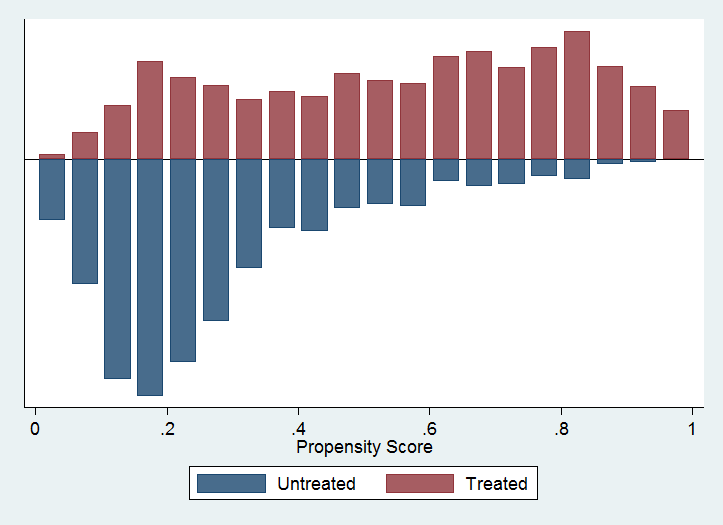
\includegraphics[width=\textwidth,trim= 0.5cm 0cm 0.5cm 0.5cm, clip=true, keepaspectratio]{common_support} \label{common_support}
\end{subfigure}

\end{figure}

To check the common support in more details I conduct balance tests, shown in Table \ref{balance}, on the matched characteristics of users and non-users of mobile money. This table reports the mean values for each covariate for users and non-users of mobile money both before and after matching was done. The t-test tests the null hypothesis that the mean value of the variable is equal for the two groups. Even after matching there are differences between users and non-users across some characteristics. In particular, per capita consumption is not equal after the match, with mobile money users always having slightly higher consumption even after matching. I look at two tests of the overall match balance, Rubins' B and R, where Rubins' B is the absolute standardised difference of the means of the linear index of the propensity score in the treated and (matched) non-treated group) and Rubin's R is the ratio of treated to (matched) non-treated variances of the propensity score index. \cite{rubin2001} suggests that the B value should be less than 25 and the R value between 0.5 and 2. After matching my B value is  28.5 which is slightly higher that ideal. My Rubins' R value is within the range suggested for a good match at 1.26. To correct for the higher per capita consumption of mobile-money-using households even after matching, I truncate the top 5\% of the consumption distribution and run my results only for the remaining 95\% of the consumption distribution. 



\begin{table}[!ht]
\centering
\resizebox{!}{0.5\textheight}{\begin{minipage}{\textwidth}
\centering
  \caption{Balance test for propensity score matching} \label{balance}
    \def\arraystretch{0.7}
    \begin{tabulary}{1\textwidth}{lCCCCC}
    \toprule
   
     &       & MM users & Non-users & t statistic  & p statistic  \\
    \midrule
    Per capita  & U     & 13.50 & 13.01 & 18.66 & 0.00   \\
        consumption  & M     & 13.50 & 13.52 & -0.44 & 0.656   \\
    
    Wealth & U     & 1.16  & -0.93 & 18.11 & 0.00    \\
          & M     & 1.15  & 1.13  & 0.12 & 0.91    \\
    Rural & U     & 0.49  & 0.79  & -16.41 & 0.00    \\
          & M     & 0.49  & 0.48  & 0.50 & 0.62   \\
    Education of  & U     & 5.96  & 3.90  & 60.10 & 0.00   \\
        head (yrs)  & M     & 5.95  & 5.97  & -0.40 & 0.94   \\
    Head female & U     & 0.22  & 0.27  & -2.22 & 0.03   \\
          & M     & 0.22  & 0.249  & -1.23  & 0.22   \\
    Age of head & U     & 44.10 & 47.26 & -5.13 & 0.00  \\
          & M     & 44.10 & 44.03 & 0.10 & 0.92    \\
    Household  & U     & 5.14  & 5.17  & -0.29 & 0.773   \\
    size      & M     & 5.14  & 4.98  & 1.14  & 0.255    \\
    Own mobile & U     & 0.69  & 0.28  & 22.05 & 0.00   \\
          & M     & 0.69  & 0.67  & 0.83  & 0.41   \\
    Number of  & U     & 0.11  & 0.05 & 4.21 & 0.00   \\
      loans    & M     & 0.11  & 0.09  & 0.93 & 0.35   \\
    Bank  & U     & 0.00  & 0.00  & .     & .      \\
        account  & M     & 0.00  & 0.00  & .     & .      \\
    ROSCA & U     & 0.07  & 0.02  & 6.30 & 0.00  \\
          & M     & 0.07  & 0.05  & 2.02 & 0.04  \\
     Agriculture/  & U     & 0.44  & 0.74  & -15.20 & 0.00   \\
        Livestock  & M     & 0.44  & 0.42  & 1.15  & 0.25   \\
     Fishing & U     & 0.01  & 0.02  & -2.19 & 0.03  \\
          & M     & 0.01  & 0.02  & -1.36  & 0.18   \\
     Mining & U     & 0.00  & 0.00  & 1.41  & 0.16   \\
          & M     & 0.00  & 0.00  & 2.00  & 0.04 \\
     Tourism & U     & 0.00  & 0.00  & .     & .     \\
          & M     & 0.00  & 0.00  & .     & .     \\
     Employed:  & U     & 0.09  & 0.03  & 6.29 & 0.00   \\
        Gov  & M     & 0.09  & 0.08  & 0.72  & 0.47   \\
     Parastatal & U     & 0.01  & 0.00  & 2.22  & 0.02   \\
          & M     & 0.01  & 0.01  & 1.50  & 0.13   \\
     Private  & U     & 0.14  & 0.04  & 8.99 & 0.00   \\
      sector    & M     & 0.14  & 0.16  & -1.60 & 0.11   \\
     NGO/ & U     & 0.01  & 0.00  & 2.68 & 0.01   \\
       religious   & M     & 0.01  & 0.03  & 0.41 & 0.68   \\
     Employed   & U     & 0.02  & 0.03  & -0.61 & 0.54 \\
       w employees   & M     & 0.02  & 0.02  & 1.54  & 0.13   \\
     Employed   & U     & 0.22  & 0.09  & 9.55 & 0.00   \\
         no employees & M     & 0.22  & 0.26  & -1.76 & 0.08   \\
    Family  & U     & 0.01  & 0.01  & -0.22 & 0.83   \\
       work   & M     & 0.01  & 0.01  & 0.83 & 0.40   \\\hline
         
    \multicolumn{6}{p{10cm}}{Matching was done on wave 1 characteristics. U is for the unmatched sample and M stands for the matched sample}
    \end{tabulary}%
    \end{minipage}}
\end{table}%


\clearpage

\subsection{Mechanisms}
In this section I examine the various mechanisms at work in this paper. I first look at the mechanism through which mobile money facilitates consumption smoothing after an aggregate shock, arguing that this is via remittances flows. I then break down the impact of mobile money by distance to the nearest mobile money agent and between urban and rural areas. I look in more detail into what is driving the negative impact of rainfall shocks by separating the impact of the shock on consumption by droughts and floods. I use a measure of rainfall as the variation from the mean to characterise non-linearities in the effect of rainfall on consumption as justification for using a 1 standard deviation as my definition of a shock. I confirm that rainfall shocks are exogenous by checking that neither of the shock variables is correlated with household demographic variables.  Finally, I examine some other aggregate shocks reported in the TNP survey to expand my results.  

\subsubsection{Remittances}
The proposed mechanism tested in this paper is that mobile money allows remittances to be sent by friends and family in other locations in response to an aggregate shock and that this allows consumption smoothing. However, it is possible that mobile money affects consumption smoothing in other ways. One possible alternative is that mobile money allows funds to be safely stored on a mobile phone as savings which can be run down in response to a shock. A second is that households might be considered more creditworthy if they use mobile money and are able to borrow more when an adverse event happens. In the TNP survey, 80\% of respondents said they send and receive money as the most important reason for using mobile money. In the third round of the survey, questions were asked on who sent remittances, by what channel, from where and what their relation was to the recipient. 40\% of remittances were sent by a son or daughter, 35\% were sent via mobile money and 30\% came form Dar es Salaam, the capital city. This suggests a story of children sending remittances home from the city via mobile money is a plausible one.  

In order to test whether remittances are driving the way that mobile money protects against adverse shocks I run the following specification: 
\begin{align}
r_{jv}=& C_{jv} + \gamma_a AggShock_{jv} + \mu MM_{jv} \notag \\ 
& + \beta_m MM_{jv}\cdot AggShock_{jv} + \bm{\theta X_{jv}} + \varepsilon_{jv} 
\end{align}
where $r_{jv}$ is the remittance amount received by a mobile money using household and the other variables are as defined previously. Log consumption per capita, $C_{jv}$, is included to control for income effects. Unfortunately, data on remittance amounts is only available for the final wave of the panel and so this specification can only be run as an OLS regression for one period. It still gives an indication though whether remittances are responding to negative shocks. If remittances are the channel through which mobile money smooths aggregate shocks then the following prediction will hold:
\begin{description}
\item{\bf{Prediction 6}} $\gamma_a>0$
\end{description}
so that remittances increase in response to an aggregate shock.   

\begin{table}
\centering 
\caption{OLS regression of remittances received after an aggregate shock} \label{remittance}
\begin{tabular}{lcc}
\multicolumn{3}{c}{Dependent variable: remittances received (Tanzania Shilling)} \\ \hline
 & (1) & (2)  \\
  & 1 sd shock & self reported shock \\ \hline
  &  &   \\
Rain shock & 34,786*** & 66,486 \\
 & (15,298) & (46,823) \\
MM use & 27,456** & 19,767* \\
 & (11,708) & (11,196) \\
Rain shock *MM use & -23,240  & 66,486  \\
 & (36,306) & (46,392)  \\
Observations & 3,311 & 3,311  \\
R-squared & 0.06 & 0.07 \\ \hline
\multicolumn{3}{p{11cm}}{Full set of control variables as in Table \ref{HH sum} and errors clustered at the village level. All regressions also control for village characteristics which could affect the ease of sending remittances. These are the distance to the nearest main road, distance to nearest population centre and distance to nearest market. MM use is a dummy variable equal to one if the household used mobile money in a given year.} \\
\multicolumn{3}{l}{ Standard errors in brackets, *** p$<$0.01, ** p$<$0.05, * p$<$0.1} \\
\end{tabular}
\end{table}
Table \ref{remittance} shows the OLS regressions of remittances received in Tanzanian Shillings in wave 3 for both self reported shocks and the 1 standard deviation rainfall shock. Remittances increase after a negative shock by 32,000-45,600 shilling (\$17-24) and this is significant at the 1\% level. Mobile money use results in the households receiving more remittances overall compared to other forms of receiving remittance \footnote{55\% of households send remittances via friends or family and 46\% via mobile money}, by between 25,500 and 46,000 shilling (\$13-25). The interaction of mobile money with the shock is not significant in either regression and is actually slightly negative in regression (2) (by 2000 shilling, \$1) though with a very large standard error. A potential reason for the high standard errors is that there are only around 100 households who reported the amount of remittances they received, experienced a rainfall shock and use mobile money  and so this result is more imprecisely estimated on a small sample\footnote{1500 households received remittances, 200 of these also experienced a rainfall shock and 100 of these use mobile money}. The results however are indicative that remittances are driving the mechanism through which mobile money smooths consumption. 

\subsubsection{The impact of distance to the mobile money agent}
The distance to the nearest mobile money agent could also impact how easy it is for someone to send and receive remittances via mobile money and hence the benefit they receive from using this service. I therefore run specification \eqref{eq: specification agg shock} with interactions with dummy variables for whether an agent is within 1km of the village, between 1km and 5km, between 5km and 10km away, with agents more than 10km away as the exclusion category. This will also indicate whether the distance to the nearest mobile money agent changes the pattern of sharing remittances within the village or the receiving household keeping the remittances. For example, it might be easier to hide remittances the further away the mobile money agent is from the village. 

The results for distance dummies interacted with each variable are reported in Table \ref{distance}. I find that having other households in the village using mobile money increases a households per capita consumption if the mobile money agent is located within 1km of the village. Since on average 1/3 of the village use mobile money if anyone does then this corresponds to an increase of 9\% per capita, a large effect. In regression (2) this result also holds for agents within 5km of the village. When a rainfall shock occurs, there is a small negative effect of other households in the village using mobile money in regression (1), but otherwise the coefficients on the shock interaction with village mobile money use are insignificant. Households using mobile money themselves benefit by between 11 and 20\% of per capita consumption when a rainfall shock occurs, more than cancelling out the negative impact of the shock of 7\%. However this effect is only strong if an agent is within 1km for regression (2) and significant at the 10\% level for agents within 5km in regression (1). 

These findings indicate that both benefit to others in the village and benefit to the user during a rainfall shock decrease the further away the mobile money agent is, with most benefits if the agent is within 1km of the village. I do not find evidence that households are sharing less with the village, and instead keeping the remittance for themselves, as the distance to the nearest mobile money agent increases. This could be because household members are less willing to walk a long distance to a mobile money agent, giving up other productive activities to do so and so are using mobile money less the further away the agent is. This could be tested if I had detailed data on the number and size of remittances received, but unfortunately I don't.   

\begin{table}
\centering \caption{Interactions with distance to the nearest mobile money agent} \label{distance}
\def\arraystretch{0.80}
\begin{tabular}{lcc} \hline
 & (1) & (2) \\
 & self reported drought or flood & 1sd rainfall shock \\ \hline
Rain shock & -0.078*** & -0.073*** \\
& (0.031) & (0.025) \\
village MM (agent 1km) & 0.252*** & 0.279*** \\
 & (0.065) & (0.067) \\
village MM (agent 5km) & 0.151 & 0.284**  \\
  & (0.156)  & (0.145) \\
village MM (agent 10km) & 0.249 & 0.047 \\
 & (0.201) & (0.203) \\
Shock*village MM (agent 1km)  & -0.016*** &  -0.009 \\
 & (0.006) &  (0.007)  \\
Shock*village MM (agent 5km) & 0.041 & -0.030 \\
 & (0.035) & (0.033)  \\
Shock*village MM (agent 10km)  & 0.036 & -0.013 \\
 & (0.060) &  (0.031) \\
MM use (agent 1km)  & 0.030 & 0.039 \\
 & (0.036) & (0.040) \\
MM use (agent 5km) & 0.050 &  0.078  \\
 & (0.085) &  (0.096)  \\
MM use (agent 10km)  & 0.094 & -0.005 \\
 & (0.095) & (0.113) \\
shock*MM use (agent 1km) & 0.204*** &  0.112**  \\
 & (0.068) &  (0.014) \\
shock*MM use (agent 5km) & 0.201* & 0.218 \\
 & (0.113) & (0.150) \\
shock*MM use (agent 10km) & 0.066 &  0.205   \\
 & (0.177) &  (0.178) \\
Observations & 8,367 & 8,367 \\
Number of households & 2,936 & 2,936 \\
R-squared & 0.287 & 0.267 \\
  \hline
\multicolumn{3}{p{14cm}}{All regressions include a full set of household control variables from table \ref{HH sum} and errors clustered at the village level.  All regressions also control for village characteristics which could affect the ease of sending remittances. These are the distance to the nearest main road, distance to nearest population centre and distance to nearest market, as well as having an ATM, bank or post office in the village.Village MM use refers to the proportion of households in the village using mobile money. MM use is a dummy variable equal to one if that household uses mobile money. The distance to the agent is a dummy variable equal to 1 if the agent is within that distance of the village.} \\
\multicolumn{3}{l}{Standard errors in brackets, *** p$<$0.01, ** p$<$0.05, * p$<$0.1} \\
\end{tabular}
\end{table}

\subsubsection{Urban-rural differences}
I run the results separately for urban and rural households to see if there are differential effects for these groups. Mobile money services would be expected to benefit rural households more since they have less access to other ways to send remittances such as banks or designated money transfer shops (such as Weston Union) and are less likely to have friends or relative passing by regularly who could bring remittances. They are also more reliant on agriculture and so affected by rainfall shocks more directly in terms of crop losses than households in urban areas. 

Separate urban and rural results are shown in in Table \ref{urban rural} where columns (1) and (3) show results for rural areas and columns (2) and (4) are for urban areas. From the results it can be seen that rainfall shocks have larger and more significant effects in rural areas than in cities, most likely because rural areas are reliant on agriculture for income making their consumption more sensitive to rainfall. The benefit from other people using mobile money in the community seems to come largely from rural areas, where with 1/3 of the village using mobile money every household benefits by 10\% of per capita consumption. In urban areas this effect is only 3\% and not significant in regression (4). When there is a rain shock, some of the benefit of having other mobile money using households in your community disappear, though this is not significant in any of the regressions.  

\begin{table}
\centering
\caption{Fixed effects regressions by urban and rural  households} \label{urban rural}
\begin{tabular}{lcccc}
\multicolumn{5}{c}{Dependent variable: Log consumption per capita} \\ \hline
& \multicolumn{2}{c}{Self reported shock} & \multicolumn{2}{c}{1sd rain shock} \\
 & (1) & (2) & (3) & (4) \\
 & rural & urban& rural & urban  \\ \hline
 &  &  &  &  \\
Rain shock & -0.07** & -0.02 &   -0.10*** & -0.07*   \\
 & (0.03) & (0.06)  & (0.04) & (0.04)  \\
Village MM use & 0.30*** & 0.11** & 0.33*** & 0.11 \\
 & (0.11) & (0.05) & (0.09) & (0.07) \\
Rain shock*village MM use & -0.20 & -0.00 & -0.16 & 0.10  \\
 & (0.16) & (0.11) & (0.13) & (0.09)  \\
MM use & -0.02 & 0.04 & -0.03 & 0.07* \\
 & (0.04) & (0.03) & (0.04) & (0.05) \\
Rain shock*MM use & 0.11* & 0.07 & 0.19** & 0.01  \\
 & (0.07) & (0.06) & (0.08) & (0.05)  \\
 &  &  &  &  \\
Observations & 6,529 & 3,241 & 6,529 & 3,241 \\
Number of households & 3,570 & 1,854 & 3,570 & 1,854 \\
R-squared & 0.10 & 0.27 & 0.10 & 0.28 \\\hline
\multicolumn{5}{p{11cm}}{Full set of control variables as in table \ref{HH sum}, household fixed effects and errors clustered at the village level. Village MM use refers to the proportion of households in the village using mobile money. All regressions also control for village characteristics which could affect the ease of sending remittances. These are the distance to the nearest main road, distance to nearest population centre and distance to nearest market, as well as having an ATM, bank or post office in the village. Mobile money use is a dummy variable equal to one if that household uses mobile money.} \\
\multicolumn{5}{l}{ Standard errors in brackets, *** p$<$0.01, ** p$<$0.05, * p$<$0.1} \\
\end{tabular}
\end{table}

Using mobile money yourself is only significant in urban areas in regression (4), giving your household an extra 6.6\% of consumption per capita. However when there is a rainfall shock it is people in rural areas who largely benefit, getting between 11 and 19\% of per capita consumption. The lack of benefit in urban areas could be because shocks are not having a significantly negative effect to begin with due to the lack of dependence of income on rainfall, or because people in cities are better protected from rainfall shocks in other ways such as from having better quality infrastructure that, for instance, prevents roads being washed away during heavy rain. These results confirm that rural households have more to gain than urban ones from increased access to mobile money services due to a combination of less methods for obtaining remittances and greater reliance on rain dependent agricultural as an income source. 

\subsubsection{Droughts and floods}
To see whether too much or too little rainfall have differential effects on consumption and the ability of mobile money to smooth these impacts, I separate out the effects of droughts compared to floods. A drought is defined as the difference in rainfall from the mean being more than one standard deviation below the mean and a flood as the difference in rainfall from the mean being more than one standard deviation above the mean. This is reported in Table \ref{Drought flood}, where droughts are reported in columns (1)-(2) and floods in columns (3)-(4), each as a simple difference-in-difference and with household fixed effects. 

It can be clearly seen that it is mainly droughts which have a significant negative effect of around 10\% of per capita consumption. Floods have no significantly different effect from zero. I perform an F test of the equality of the drought and flood effects. Equality is rejected at the 1\% level  for the simple difference-in-difference specification but only at the 10\% level for the regression with household fixed effects. Hence there is some evidence for differential effects of droughts and floods, with droughts primarily negatively affecting consumption. Having other people in the village use mobile money is significant in all the regressions. At the mean of 1/3 of people using mobile money in the village, consumption per capita is between 7 and 9\% higher. Mobile money use is only significant in the simple difference-in-difference specification, increasing consumption per capita by 13-15\%, but this effect goes to 5\% once household fixed effects are accounted for. Looking at the shock interactions, other people in the village using mobile money during a shock is not significant in any of the regressions. The shock interacted with a household's own mobile money use is significant in both of the drought regressions at the 10\% level. 

These results confirm my earlier findings but reveal that it is only droughts that actually cause a reduction in per capita consumption. Mobile money increases per capita consumption after a rainfall shock only when a drought  occurs, not when a flood occurs, which makes sense since floods aren't causing a drop in consumption to begin with. These results also link with the earlier finding that it is mainly rural households who experience a drop in consumption after a rainfall shock and benefit most from mobile money. Rural households are likely to be most affected by a drought since it directly reduces their income through crop losses, whereas urban households will only be affected indirectly. These results therefore support each other. The lack of impact of floods might also indicate the presence of non-linearities in the impact of rainfall, with too much rain initially increasing crop yields, whereas too little rain always has a negative impact on crop yields. I examine possible non-linearities in more detail below.

\begin{table}
  \centering
  \caption{Differential impacts of droughts and floods} \label{Drought flood}
\begin{tabulary}{1\textwidth}{Lcccc} \multicolumn{5}{c}{Dependent variable: Log consumption per capita} \\\hline
& \multicolumn{2}{c}{Drought} & \multicolumn{2}{c}{Flood} \\ \cmidrule(r){2-3} \cmidrule(l){4-5}
 & (1) & (2) & (3) & (4)  \\
VARIABLES & Diff-in-diff & FE  & Diff-in-diff & FE \\ \hline
 &  &  &  &    \\
Shock & -0.10*** & -0.11*** & 0.02 & -0.01   \\
 & (0.03) & (0.03) & (0.03) & (0.03)  \\
Village MM use & 0.12** & 0.23***  & 0.10* & 0.27**  \\
 & (0.05) & (0.04)  & (0.06) & (0.13) \\
Shock*village MM use & 0.19 & 0.07  & -0.01 & -0.06   \\
 & (0.16) & (0.17)  & (0.08) & (0.08)  \\
MM use & 0.15*** & 0.05*  & 0.13*** & 0.05*  \\
 & (0.02) & (0.02)  & (0.03) & (0.03)  \\
Shock*MM use & 0.10* & 0.14*  & 0.06 & 0.01  \\
 & (0.06) & (0.08)  & (0.04) & (0.05)  \\
Observations & 9,770 & 9,770  & 9,770 & 9,770\\
Number of households  & 3,798 & 3,798 & 3,798 & 3,798 \\
R-squared & 0.57 & 0.13  & 0.55 & 0.08  \\ \hline

 F stat on equality & 7.19 &  3.36 & & \\
 p value & 0.008 &  0.067 & & \\
 \hline
\multicolumn{5}{p{12cm}}{All regression include a full set of control variable from Table \ref{HH sum}, time dummies and clustered errors at the village level. Village MM use refers to the proportion of households in the village using mobile money. All regressions also control for village characteristics which could affect the ease of sending remittances. These are the distance to the nearest main road, distance to nearest population centre and distance to nearest market, as well as having an ATM, bank or post office in the village. Mobile money use is a dummy variable equal to one if that household uses mobile money. The F stat is a test of equality of the drought and flood coefficients for the diff-in-diff and fixed effects regressions. The resulting p value is reported as well. } \\
\multicolumn{5}{l}{ Standard errors in brackets, *** p$<$0.01, ** p$<$0.05, * p$<$0.1} \\
\end{tabulary}
\end{table}

\subsubsection{Non-linearities in rainfall shocks}
Rainfall shocks have very non-linear effects, with a little more rain often good for crops but only extreme amounts harmful, and likewise a little less rain unlikely to cause much hardship whereas a drought would cause widespread crop damage. I use deviations of rainfall from the mean to check for non-linear effects of the rainfall shock magnitude, and this is reported in Table \ref{Rain dev}. In this table I look at the deviations of rainfall from the mean and the square of this to find any turning points in the impact of rainfall on per capita consumption. Column (1) shows the results for both positive and negative deviations, whereas column (2) only looks at deviations below the mean and column (3) at deviations above the mean. 

It can be seen in column (2) that negative shocks always have a negative effect on consumption, with 200mm less rain in the year reduced consumption by 9.2\%. More rainfall initially has a positive effect on log consumption per capita but this becomes negative for rainfall more than 300mm above the mean, with 500mm more rainfall than usual reducing log consumption by 4.2\%. This shows that while droughts always have a negative impact on per capita consumption, more rain initially has a positive impact and it is only sufficiently extreme rainfall that has a negative effect. 
\input{rain_dev}

\subsubsection{Exogeneity of rainfall shock}
I confirm the exogeneity of the rainfall shock by showing that the rainfall shock is not correlated with any characteristics of the households. Fixed effect regressions for each of the rainfall shocks are shown in Table \ref{shock corr}. In column (1), the 1 standard deviation rainfall shock, only using a ROSCA is significant at the 10\% level. For the self reported rainfall shocks in column (2), ROSCA is again significant at the 10\% level but has the opposite sign from the regression in column (1). The agriculture household head occupation dummy is also significant at the 10\% level with working in agriculture associated with a 9\% higher probability of reporting a shock, possibly because the household is more sensitive to the weather if they work in agriculture. Overall these results suggest my rainfall shock variables are not correlated with characteristics of the households. 


\begin{table}
\centering \caption{Shock correlations} \label{shock corr}
\def\arraystretch{0.7}
\begin{tabular}{lcc} \hline
 & (1) & (2) \\
 & Self reported drought/flood  & 1sd rain shock \\ \hline
Rural& -0.027** & -0.046 \\
 & (0.013) &(0.048) \\
Wealthscore & 0.004*** & 0.002 \\
 & (0.001) & (0.012) \\
Head education & -0.001 & 0.029*** \\
 & (0.002) & (0.011)  \\
Head age & -0.003 & 0.001 \\
 & (0.002) & (0.002) \\
Household size & 0.005  & 0.023** \\
 & (0.004) & (0.010) \\
Mobile phone & 0.012 & 0.077 \\
 & (0.013) & (0.077)\\
Loan & 0.022 & -0.127 \\
 & (0.015) & (0.101) \\
Bank account  & -0.026**  & -0.089\\
 & (0.012)  & (0.100)  \\
ROSCA & 0.026 & -0.547*** \\
 & (0.030)  & (0.172)  \\
Agriculture & 0.045 & 0.230  \\
 & (0.033) & (0.180)  \\
Fishing  & 0.062 & 0.049  \\
 & (0.041) & (0.273) \\
Government  & 0.030 & 0.024 \\
 & (0.049)& (0.232)  \\
Parastatal & 0.008 & -0.717 \\
 & (0.057)  & (0.476) \\
Private sector  & -0.006 & 0.177 \\
 & (0.027) & (0.212) \\
NGO/Religious & -0.034 & -0.053\\
 & (0.056)  & (0.431) \\
Self employed & 0.001 & 0.202\\
 & (0.025)  & (0.203) \\
Family work& -0.008  & 0.644*\\
 & (0.029)  & (0.355) \\
Unemployed & 0.013 & 0.262\\
 & (0.037) & (0.736)  \\
Observations & 9,281 & 1,090 \\
R-squared & 0.056 & 0.114 \\ \hline
\multicolumn{3}{p{12cm}}{Regression one has village fixed effects and is at the village level for village averages of the household characteristics, since the one standard deviation rainfall shock is constant for a village. Regression two has household fixed effects and village clustered errors and is at the household level since each household reports whether it experienced a shock or not.  } \\
\multicolumn{3}{l}{ Standard errors in brackets, *** p$<$0.01, ** p$<$0.05, * p$<$0.1} \\
\end{tabular}
\end{table}
 
\subsubsection{Other shocks}
Finally I check whether the results found are particular to floods and droughts or also extend to other aggregate shocks. The theoretical predictions I made based on equation \eqref{eq: specification agg shock} apply to any aggregate shock, not only rainfall shocks, and so I check that my results generalise by running this specification again with different aggregate shock measures. These results are reported in Table \ref{other shocks}. I have self-reported data on three other aggregate shocks: Large fall in crop prices, large rise in food prices and large rise in agricultural input prices. 

None of the three shocks have a significant negative effect on per capita consumption. However, when a shock occurs, those using mobile money themselves experience a 16\% increase in per capita consumption in two of the regressions despite the shock not causing a fall in consumption. Regression (2) may not show a significant effect because 40\% of people in the sample reported experiencing large rises in food prices so this shock affects large numbers of people across the country at the same point in time, making it less likely someone not experiencing this shock could support someone experiencing it. Other people in the village using mobile money still has a highly significant 8\% increase on per capita consumption ($1/3$ of 17\%), similar to that found before. 

Overall then, these results provide support that my main findings using rainfall extend to any aggregate shocks, not just rainfall shocks, but suggest it might be rainfall shocks which households currently have the most difficulty smoothing themselves. 

\begin{table}
\centering \caption{Diff-in-diff fixed effect regressions of other aggregate shocks on consumption} \label{other shocks}
\begin{tabular}{lccc} 
\multicolumn{4}{c}{Dependant variable: Log consumption per capita}\\ \hline
 & (1) & (2) & (3) \\
 & Large fall crop price & Large rise food price & Large rise agri input price \\ \hline
Shock & 0.09*** & 0.01  & 0.07***  \\
 & (0.02) & (0.03)  & (0.03)  \\
Village MM use & 0.10* & 0.06 & 0.11** \\
 & (0.05) & (0.06) & (0.05) \\
Shock*village MM & -0.24*** & 0.07   & -0.25  \\
 & (0.13)  & (0.07)  & (0.10) \\
Mobile money use & 0.04 & 0.05 & 0.03 \\
 & (0.02) & (0.03) & (0.03) \\
Shock*MM use & 0.10* & -0.01  & 0.15***
  \\
 & (0.07) & (0.04)  & (0.05) \\

Observations & 7,704 & 7,704 & 7,704 \\
R-squared & 0.178 & 0.176 & 0.178 \\
Number of households & 3,032 & 3,032 & 3,032 \\
  \hline
Mean of User & 0.118 & 0.118 & 0.118 \\
 Mean of Shock & 0.123 & 0.423 & 0.121 \\ \hline
\multicolumn{4}{p{14cm}}{ All regressions include full set of household control variables from Table \ref{HH sum}, household fixed effects and errors clustered at the village level. All regressions also control for village characteristics which could affect the ease of sending remittances. These are the distance to the nearest main road, distance to nearest population centre and distance to nearest market. Village MM use refers to the proportion of households in the village using mobile money. Mobile money use is a dummy variable equal to one if that household uses mobile money. } \\
\multicolumn{4}{l}{ Standard errors in brackets, *** p$<$0.01, ** p$<$0.05, * p$<$0.1} \\
\end{tabular}
\end{table}

\subsection{Discussion} 
This paper is a contribution to the early literature on mobile money because it both confirms an earlier finding that mobile money helps households smooth  shocks (Jack \& Suri 2014) and extends this analysis to the wider impact on the rest of the community from having mobile money users in the village. Looking at just the impact on the user of mobile money would therefore underestimate the benefits of having mobile money in a community. Benefits to both the user and community are highest in rural areas and decrease sharply with distance to the nearest mobile money agent. Efforts to facilitate the spread of mobile money agents to more communities would increase welfare, especially since the more remote the community the less likely the community has other ways to receive remittance and so the larger the benefits from having mobile money services could be. 

The fact that mobile money increases average village consumption but only helps the recipient household smooth consumption after an aggregate shock is an important contribution to the risk sharing literature. Exploring why this is the case would advance our understanding of how informal risk sharing arrangements operate in developing countries. For example, are households choosing to hide remittances or are they opting out entirely from the risk sharing network in the village? Looking at transfers within the village and from a migrant in response to idiosyncratic shocks would allow these effects to be separated. My data was not detailed enough on specific network patterns and remittance flows to answer this question, but the answer is important for understanding how new technologies change traditional risk sharing patterns and for a deeper understanding of how risk sharing networks are sustained.  

There are many potential explanations for why remittances might not be shared after an aggregate shock. \cite{coate1993} looked at risk sharing as a repeated game and determined the conditions under which an informal risk sharing network is self-sustaining. To be self-sustaining, at every point in time the benefits from remaining in the relationship must outweigh the benefit of defection. These conditions include the ability to punish  deviations from risk sharing which requires information on network members. In regards to mobile money, information on the amount of money received may be hard for other villagers to obtain, particularly if the mobile money agent is outside the village itself. Without accurate information on if remittances have been received and the amount, it is very hard for the rest of the villagers to ask for more transfers when a shock has occurred or to punish the mobile-money-using household for not sharing remittances. Differences in the impact of an aggregate shock on each individual household also creates uncertainty for households to know the extend to which other households' consumption falls after a village level shock. Again this means other households in the village cannot be sure that a mobile money using household is smoothing its consumption due to remittances received or because it simply suffered less from the aggregate shock by chance. 

Secondly, the benefit from defection might increase for a mobile-money-using household, because they can then keep any remittances received for themselves at every point in time. They could insure both aggregate and idiosyncratic shocks through the migrant, and the benefits of this risk sharing relationship might exceed those of the village risk sharing relationship. In this case, mobile money using households might no longer participate at all in village risk sharing. However, it is unclear then why I find that having a household using mobile money in the village  benefits every other households if the mobile-money-using household is not sharing remittances at all.  

Another reason why remittances aren't shared after an aggregate shock is that norms for sharing in the village don't extend to aggregate shock. Norms develop to address situations which an individual cannot solve alone but that the village as a whole can overcome. Traditionally, the norm has been that only individual shocks are shared by the village. Aggregate shocks were not shared because they impacted the entire village at once and so could not be smoothed. The introduction of mobile money has enabled households to have links with other households in other locations and hence for some households in a village to smooth aggregate shocks. However the social norm might still required households to only share income for idiosyncratic shocks, not aggregate. Hence there is no requirement for households to share income after an aggregate shock, explaining why I don't see sharing in the data. However there is a norm that households pool their income when an aggregate shock has not occurred, resulting in mobile-money-using households sharing remittances and overall village consumption being higher.

\cite{coate1993} also showed that after a big event like a famine in which incomes fall substantially, the discount factor required for a household to remain in a risk sharing arrangement goes up as the income of the others goes down. This results in the break down of informal risk sharing relationships if the contribution of a relative fortunate household is insufficient to keep the other households from starvation. It is possible that a similar situation occurs after an aggregate shocks, with some households experiencing larger income falls than others and risk sharing breaking down temporarily.  

The literature on risk sharing has often found that risk sharing isn't necessarily taking place at the village level but instead in sub-networks within the village and with networks of family and friends outside the village (Fafchamps \& Lund 2003, De Weerdt \& Dercon 2006). If this is the proper network over which risk sharing takes place, I might not find sharing at the village level to aggregate shocks when in fact there is risk sharing occurring within sub-networks that extend beyond the village. It therefore appears as though mobile money users are keeping remittances themselves after an aggregate shock when in fact they are sharing across villages. It would be an interesting piece of further work to examine in detail the networks of mobile money users and non users to find out how they overlap and address this question. 

A final reason for lack of sharing of remittances after an aggregate shock could be due to pressure from the migrant to prevent the receiving household from sharing any additional remittances with other households in the village. If the migrant is already sending a steady stream of remittances to the household in the village and is then asked to send more because of a rainfall shock, they might only send more remittances conditional on these not being shared with the rest of the village. The migrant is not in the risk sharing network with the rest of the village and so has no desire to have additional transfers shared with the entire village. I also assumed that the migrant knew accurately the consumption of the receiving household and the average shortfall due to an aggregate shock. Hence the migrant would only send enough to allow that one household to smooth consumption, not enough to share with the entire village.  

While all of these explanations are possible, it would be interesting future work to examine them in detail and determine which are the strongest effects. This links into the question of determining how, if at all, improved access to remittances changes traditional risk sharing networks in villages, for better and for worse. 






\newpage
\clearpage
\section{Conclusion}
Even if idiosyncratic shocks are shared perfectly within the village, households in developing countries are still subject to large changes in consumption due to aggregate shocks, such as rainfall shocks, which negatively affect the consumption of the entire village at one. Droughts and floods are a major source of risk to developing households, and measures which help protect against these, ranging from social protection to micro-insurance, are key areas of research. Mobile money services are a new and fast growing technology which can help households insure their consumption against aggregate shocks by providing access to remittances.

In this paper I show that idiosyncratic shocks are perfectly insured at the village level but that large rainfall shocks negatively affect household consumption, therefore confirming the predictions of the Mace (1991) model. I then look at the impact mobile money use has on consumption in communities with mobile money, comparing users and non-users. I find that consumption per capita is higher for all households in communities with mobile money. However, when it comes to smoothing aggregate shocks, only mobile money users are  able to smooth their consumption after the shock. 

I confirm the robustness of my findings using a placebo test from before the introduction of mobile money to test the common trends assumption, instrumental variable techniques to address potential self-selection effects into mobile money use and propensity score matching to overcome selection bias based on observable covariates. All of these confirm my results. 

I check the proposed mechanism that the consumption smoothing effect is due to households that use mobile money receiving remittances, by looking at the value of remittances received in the final wave of data. I look at the correlation of migration with having a mobile money agent in the village, and the impact of distance to the nearest agent on consumption smoothing after an aggregate shock. I extend my results by looking at urban and rural households and droughts and floods separately. I find suggestive evidence that it is principally rural mobile-money-using households that benefit from improved ability to smooth rainfall shocks and who also share remittances with their communities when an aggregate shock hasn't occurred. It is principally droughts which negatively affect consumption and that are smoothed when a household uses mobile money. I also confirm my results extend to other types of aggregate shock.  

Research on the impact of mobile money services is still in its infancy. Further work could explore in more detail how access and use of mobile money services changes traditional risk sharing arrangements and who the winners and losers are from this. While this work has looked at the benefits of mobile money services at the level of the household, interesting further work would examine how these benefits are distributed within the household and how mobile money services affect intra-household decision making. 





\clearpage
\bibliographystyle{apalike}
\bibliography{Bibliography}
%\appendix
\section{Village mean characteristics}
\begin{table}[htbp] 
  \centering
  \caption{Village characteristics} \label{village sum}
    \begin{tabular}{lrrrrrr}
    \toprule
          & Wave 1 &       & Wave 2 &       & Wave 3 &  \\
    \midrule
     Service     & Mean  &  SD   & Mean  &  SD   & Mean  &  SD  \\
  
    ATM   & 0.00  & 0.00  & 0.07  & 0.26  & 0.10  & 0.30 \\
    Bank  & 0.08  & 0.28  & 0.06  & 0.24  & 0.09  & 0.28 \\
    Community/public owned tap water & 0.45  & 0.50  & 0.34  & 0.47  & 0.41  & 0.49 \\
    Court & 0.11  & 0.32  & 0.12  & 0.32  & 0.14  & 0.35 \\
    health\_centre&    0.51&    0.50 & 0.54 & 0.25 &0.56  & 0.25 \\
hospital    &    0.09&     0.29 & 0.08 & 0.07 & 0.09 & 0.08 \\
    Market daily & 0.25  & 0.43  & 0.25  & 0.44  & 0.26  & 0.44 \\
    Market weekly & 0.18  & 0.38  & 0.19  & 0.40  & 0.22  & 0.42\\
    Mobile money agent point & 0.00  & 0.00  & 0.17  & 0.38  & 0.51  & 0.50 \\
    Mobile money access  & 0.00  & 0.00  & 0.38  & 0.49  & 0.64  & 0.48 \\
   
    Police station & 0.20  & 0.40  & 0.18  & 0.39  & 0.22  & 0.41 \\
    Post office & 0.08  & 0.27  & 0.06  & 0.23  & 0.08  & 0.26 \\
    Pre-primary school/nursary & 0.63  & 0.48  & 0.72  & 0.45  & 0.86  & 0.35 \\
    Primary market for livestock & 0.03  & 0.16  & 0.05  & 0.22  & 0.18  & 0.39 \\
     Primary school&    0.86&    0.34 & 0.82 & 0.15 & 0.88 & 0.11\\
Secondary school&    0.41&   0.49& 0.47 &0.25 &0.48 & 0.25\\SACCOs & 0.36  & 0.48  & 0.35  & 0.48  & 0.34  & 0.47 \\
    \bottomrule
    \multicolumn{7}{p{13cm}}{Average characteristics for the 409 communities in each wave. Mobile money access refers to a mobile money agent within 5km of the community.}
    \end{tabular}%
  \label{tab:addlabel}%
\end{table}%

\end{document}